% Revision based on the author's re-supplied submitted manuscript (2026-11-10).
% Edits are limited to editor/reviewer concerns and demonstrable errors.
% Existing red revisions are retained; blue identifies corrections in the latest rounds.

\documentclass[final,5p]{elsarticle}
\ifdefined\pdfobjcompresslevel
  \pdfobjcompresslevel=0
\fi
\usepackage{amsmath,amssymb,amsfonts}
\usepackage{microtype,pifont}
\usepackage{graphicx}
\usepackage{dblfloatfix}
\usepackage[dvipsnames]{xcolor}
\usepackage{pgfplots}
\usepgfplotslibrary{groupplots}
\pgfplotsset{compat=1.18}
\usepackage{booktabs,multirow,tabularx,array,makecell}
\usepackage{algorithm,algorithmicx,algpseudocode}
\usepackage{enumitem, float,placeins}
\usepackage{caption}
\usepackage[colorlinks,bookmarksopen,bookmarksnumbered,citecolor=blue, colorlinks=true,linkcolor=blue,urlcolor=blue,breaklinks=true]{hyperref}
% \hypersetup{pdfstringdefDisableCommands={\def}}
\usepackage{xurl}
\usepackage{orcidlink}
\usepackage{balance}
% Permit top/bottom placement of two-column floats and reduce float starvation.
\setcounter{topnumber}{3}
\setcounter{dbltopnumber}{3}
\renewcommand{\topfraction}{0.9}
\renewcommand{\dbltopfraction}{0.9}
\renewcommand{\bottomfraction}{0.8}
\renewcommand{\textfraction}{0.05}
\renewcommand{\floatpagefraction}{0.75}
\renewcommand{\dblfloatpagefraction}{0.75}
% \setlength{\emergencystretch}{3em}
% \Urlmuskip=0mu plus 1mu

% =========================
% Commands and styles
% =========================
\newcommand{\cmark}{\textcolor{ForestGreen}{\ding{51}}}
\newcommand{\xmark}{\textcolor{BrickRed}{\ding{55}}}
% Revision markup for the FGCS major revision. Remove \rev/\begin{revision} wrappers after acceptance if desired.
\newcommand{\rev}[1]{\textcolor{BrickRed}{#1}}
\newcommand{\newrev}[1]{\textcolor{blue}{#1}}

\newcolumntype{R}[1]{>{\raggedleft\arraybackslash}m{#1}}
\newcolumntype{L}[1]{>{\raggedright\arraybackslash}m{#1}}
\newcolumntype{C}[1]{>{\centering\arraybackslash}m{#1}}

\renewcommand{\algorithmicrequire}{\textbf{Input:}}
\renewcommand{\algorithmicensure}{\textbf{Output:}}
\algrenewcommand\algorithmiccomment[1]{\hfill{\footnotesize$\triangleright$ #1}}

\makeatletter
\newcommand{\algorithmautorefname}{Algorithm}
\renewcommand{\figureautorefname}{Figure}
\renewcommand{\tableautorefname}{Table}
\renewcommand{\equationautorefname}{Eq.}
\renewcommand{\sectionautorefname}{Section}
\makeatother

\journal{Future Generation Computer Systems}
% \journal{Computer Networks}

\begin{document}

\begin{frontmatter}

\title{AIO-Mesh: Hardware-Safe AIOps Orchestration for Cloud-Native Distributed Services over Programmable Infrastructures}

\author[add1]{Hanh P. Du\orcidlink{0000-0002-8993-1164}}
\ead{hanhdp@vnu.edu.vn}

\author[add1]{Hung D. Hoang\orcidlink{0009-0004-2310-3536}}
\ead{22028293@vnu.edu.vn}

\author[add2]{Thu H. Le\orcidlink{0009-0006-4295-850X}}
\ead{lehthub1@gmail.com}

\author[add2]{Tuan X. Le\orcidlink{0009-0004-5070-9533}}
\ead{tuanlx.psa@gmail.com}

\author[add3]{Giang L. Nguyen\orcidlink{0000-0001-6184-1469}}
\ead{nlgiang@ioit.ac.vn}

\author[add1]{Hoa N. Nguyen\orcidlink{0000-0002-2565-281X}\corref{cor1}}
\ead{hoa.nguyen@vnu.edu.vn}

\cortext[cor1]{Corresponding author}

\affiliation[add1]{
organization={Department of Information Systems, VNU University of Engineering and Technology},
city={Hanoi},
postcode={11314},
country={Vietnam}
}
\affiliation[add2]{
organization={National Data Center, Ministry of Public Security},
city={Hanoi},
postcode={11309},
country={Vietnam}
}
\affiliation[add3]{
organization={Institute of Information Technology, Vietnam Academy of Science and Technology},
city={Hanoi},
postcode={11355},
country={Vietnam}
}



\begin{abstract}
Cloud-native distributed infrastructures increasingly integrate Kubernetes-based lifecycle management, service-chain orchestration, software-defined control, and programmable data planes. \rev{Artificial intelligence for IT operations (AIOps) can support online orchestration, but policy decisions may remain non-deployable because of hard CPU, memory, and Segment Routing over IPv6 (SRv6) Maximum Segment Depth (MSD) constraints.} This paper presents AIO-Mesh, a hardware-safe AIOps \rev{runtime that integrates telemetry-driven policy inference, independent admission and resource reservation, virtual network function (VNF) lifecycle management, SRv6/P4 steering, and data-plane feedback.} \rev{Its replaceable Hardware-Aware Reinforcement Policy (HARP) combines graph-attention encoding, MaskablePPO, hard action masking, and adaptive penalties to select compact placement--routing pairs.} \rev{AIO-Mesh separates hard deployability constraints from soft operational objectives through policy-side masking, independent pair-level admission, and realization-time validation of modeled CPU, memory, and per-profile MSD constraints before actuation.} Experiments on the Vietnam, NSFNET, and GEANT2 topologies \rev{using 20 matched simulation seeds with a fixed HARP checkpoint show that HARP outperforms conventional baselines and achieves statistically significant safe-acceptance gains over a feasibility-aware heuristic in seven of nine comparisons.} Under Burst Surge, HARP achieves safe acceptance rates of \rev{$19.15\pm0.46\%$} on Vietnam and \rev{$50.25\pm0.44\%$} on GEANT2. \rev{Hardware-in-the-loop experiments integrating MicroK8s, Tekton, Mininet, BMv2, and SRv6/P4 steering report zero observed admitted MSD violations under protected execution. These results remain conditional on the modeled checks and controller-visible state, without establishing unconditional full-chain deployability or atomic cross-controller execution.}
\end{abstract}



\begin{keyword}
AIOps \sep Cloud-native distributed services \sep Hardware-safe orchestration \sep Service function chaining \sep Network function virtualization \sep Programmable infrastructures \sep SRv6 \sep P4 \sep Safe reinforcement learning \sep Runtime admission control
\end{keyword}

\end{frontmatter}

\section{Introduction}
\label{sec:introduction}

Future cloud-native infrastructures are becoming distributed, programmable, and operationally dynamic. Modern service platforms combine Kubernetes clusters, edge and regional compute sites, software-defined networking, telemetry pipelines, workflow engines, and programmable forwarding devices. These infrastructures no longer host only conventional microservices; they increasingly host network and security services such as firewalls, intrusion detection systems, load balancers, deep packet inspection functions, gateways, and other virtualized or containerized network functions. In security-oriented service chains, these functions may also include AI-powered traffic inspection and intrusion-detection modules; prior studies on large-scale traffic sensing, real-time intrusion detection, and hybrid signature--deep analysis pipelines show that such AI-enabled security functions are increasingly deployable as operational traffic-processing services~\cite{cSDAID22}. Such functions are composed into service chains to enforce traffic-processing policies across tenants, applications, and security domains. As a result, infrastructure operation requires continuous decisions about where to place service functions, how to steer traffic through them, when to migrate overloaded instances, and how to preserve service objectives under changing demand, heterogeneous resources, and topology-dependent latency.

This problem is naturally an \rev{artificial intelligence for IT operations (AIOps)} problem rather than a one-shot optimization problem. In a production cloud-native environment, orchestration decisions are made from telemetry, policy intent, service demand, resource state, and runtime feedback. A learned policy must also be operated as a managed artifact: it must be loaded with the correct topology and normalization state, invoked through a stable inference path, monitored during execution, constrained by safety checks, and connected to cloud-native and network-control actuators. This view is consistent with recent \rev{machine learning operations (MLOps)} and AIOps literature, which emphasizes that machine-learning models must move from isolated training pipelines into monitored, versioned, trustworthy, and feedback-driven operational loops~\cite{kreuzberger2023mlops,diazdearcaya2024joint,eken2025mlops,bayram2025trustworthy,zhang2025aiopsllm,eramo2024architecture}. In infrastructure orchestration, however, the runtime faces an additional challenge: an AI decision may be valid in a logical model but non-deployable on the physical or programmable substrate.

Programmable data planes make this deployability gap explicit. Segment Routing over IPv6 (SRv6) allows an ingress node to encode a list of Segment Identifiers (SIDs) in the packet header, enabling stateless traffic steering through paths and service functions~\cite{filsfils2015segment,rfc8986,rfc9352}. P4-programmable switches expose packet-processing behavior through programmable parser, match-action, and deparser stages~\cite{jeyakumar2014p4}. Together, SRv6 and P4 provide a practical substrate for steering cloud-native service chains without maintaining per-flow state at every intermediate node. Yet this flexibility is bounded by hardware. A programmable parser can inspect only a limited number of SIDs in a single pass. This limit, commonly represented by the Maximum Segment Depth (MSD), is not a tunable preference but a hard parsing boundary. If a selected service path requires a SID stack deeper than the supported MSD of the relevant forwarding profile, the action is not merely suboptimal; it is not admissible. \rev{Unchecked overflow may cause installation rejection, parser errors, or packet drops, depending on the forwarding target.}

Existing orchestration methods do not fully address this operational safety requirement. Classical \rev{integer linear programming (ILP)} and heuristic formulations provide useful models for service-chain placement and routing, but they \rev{may incur high solution cost or sacrifice global optimality in online operation}. Recent \rev{deep reinforcement learning (DRL)} and graph-based methods improve adaptive \rev{service function chaining (SFC)} embedding and \rev{virtual network function (VNF)} placement~\cite{wang2021drl,xiao2023twostage,liu2024sfcml,taktak2024drl,wu2025drl}, and migration-oriented studies address failure prediction, load pressure, and migration budgets~\cite{zhai2023migration,addad2022ai,qin2023sfcmigrationbudget,afrasiabi2024cluster,zhang2025sfcmigration,hu2026rlpmo}. SRv6-aware approaches such as SFCPlanner show the relevance of source-routed flow steering for service-chain planning~\cite{qiu2024sfcplanner}. \rev{Safe reinforcement learning, shielding, and invalid-action masking also provide established mechanisms for restricting unsafe actions~\cite{alshiekh2018shielding,gu2024safe,wachi2024constraint,huang2022closer}. However, their applicability to programmable orchestration depends on whether the checked policy action corresponds to the realized forwarding configuration.} This is \rev{important} for AIOps control, where unsafe actuation can convert a policy error into a data-plane failure.

The core research question addressed in this paper is therefore: \rev{\emph{how can an AIOps runtime use learned policies for cloud-native distributed service orchestration while independently checking hardware deployability before actuation?}} This question has three coupled challenges. First, the decision policy must be topology-aware because placement, routing, SID depth, and latency depend on the structure of the substrate graph. Second, the runtime must distinguish hard deployability constraints from soft operational objectives. CPU, memory, and MSD feasibility must be enforced before actuation, whereas latency, service-level pressure, and \rev{action-switching cost} can be optimized through the reward function. Third, the learned policy must be embedded into a closed-loop AIOps runtime that connects telemetry, state construction, inference, safety validation, cloud-native lifecycle management, programmable steering, and feedback monitoring.

To address these challenges, we propose \textbf{AIO-Mesh}, a hardware-safe AIOps orchestration framework for cloud-native distributed services over programmable infrastructures. AIO-Mesh treats the learned policy as one component of an operational control loop rather than as a standalone optimizer. Its runtime integrates telemetry-driven state construction, policy inference, hard-feasibility validation, smart admission control, Kubernetes/Tekton-based VNF lifecycle actions, SRv6/P4 steering, and data-plane feedback. At the core of AIO-Mesh, we introduce \textbf{HARP} (\textbf{H}ardware-\textbf{A}ware \textbf{R}einforcement \textbf{P}olicy), a graph-reinforcement policy for \rev{topology-aware placement--routing selection}. HARP combines graph-attention topology encoding, \rev{masked Proximal Policy Optimization (PPO)}, invalid action masking, adaptive penalties for soft service objectives, and explicit \texttt{NO\_SAFE\_ACTION} handling under saturation. \rev{Its proposals pass through a policy-independent runtime admission boundary; migration is managed by the lifecycle workflow.}

The main contributions of this paper are summarized as follows.

\begin{itemize}
    \item We formulate hardware-safe AIOps orchestration for cloud-native distributed service chains over programmable infrastructures, explicitly separating hard deployability constraints from soft operational objectives. In this formulation, SRv6 MSD feasibility is treated as an admission condition rather than a reward penalty.

    \item We design \textbf{AIO-Mesh}, a closed-loop AIOps runtime that operationalizes a learned policy through telemetry ingestion, normalized state construction, inference serving, safety validation, cloud-native lifecycle management, programmable SRv6/P4 actuation, and runtime feedback.

\item We propose \textbf{HARP}, a hardware-aware reinforcement policy that combines graph-attention topology encoding, masked policy optimization, \rev{and adaptive operational penalties for topology-aware placement--routing selection}.

\item We \rev{integrate hardware-aware action masking with policy-independent runtime admission: masking filters locally infeasible candidates before sampling, whereas admission checks proposals before actuation and returns \texttt{NO\_SAFE\_ACTION} when no candidate passes the implemented checks}.

    \item We evaluate AIO-Mesh through multi-topology stress simulations and a hardware-in-the-loop cloud-native testbed integrating MicroK8s, Tekton, Mininet, BMv2 P4 switches, SRv6 steering, and telemetry feedback. The evaluation distinguishes pre-admission unsafe candidates from admitted data-plane violations, which is essential for interpreting safety-preserving rejection under saturation.
\end{itemize}

\section{Background and Related Work}
\label{sec:related}

This section positions AIO-Mesh at the intersection of AIOps, cloud-native resource orchestration, service function chaining, programmable data planes, and safe reinforcement learning. The key distinction is that AIO-Mesh is not only a placement or routing algorithm. It is an AIOps runtime in which a learned policy must be observed, constrained, admitted, actuated, and verified before it changes the state of a programmable distributed infrastructure.

\subsection{AIOps and MLOps for Cloud-Native Infrastructure}
\label{subsec:related_aiops}

AIOps applies AI techniques to the operation of complex software and infrastructure systems. Typical tasks include anomaly detection, failure prediction, incident triage, capacity planning, root-cause analysis, and automated remediation. Recent AIOps and MLOps surveys emphasize that modern operational systems rely on heterogeneous telemetry and increasingly require closed-loop workflows rather than isolated predictive models~\cite{diazdearcaya2024joint,zhang2025aiopsllm}. MLOps complements this view by addressing the lifecycle of machine-learning artifacts, including model packaging, versioning, deployment, inference serving, monitoring, robustness, and rollback~\cite{kreuzberger2023mlops,eken2025mlops,bayram2025trustworthy}.

For cloud-native infrastructures, this operational perspective is essential. Placement, migration, scaling, and steering decisions are not made once; they are continuously revised as traffic demand, resource pressure, and service objectives change. Recent work on intelligent DevOps automation, Kubernetes-oriented microservice placement, elastic container management, dynamic cloud resource allocation, and computing-continuum resource selection similarly argues that automation systems must connect models, runtime evidence, and deployment actions~\cite{eramo2024architecture,ding2023kubernetes,mao2023flowcon,chen2023workloadwindows,chen2024crossedge,sedghani2024space4aid}. AIO-Mesh follows this direction but focuses on a harder class of actuation: the policy output directly affects VNF lifecycle, traffic steering, and programmable data-plane behavior. Therefore, the runtime must be fail-closed and safety-aware, not merely prediction-driven.

\begin{table*}[t]
\centering
\caption{Positioning of AIO-Mesh against representative related work. \rev{The MSD column concerns explicit SRv6 admission, not general resource-constraint handling.}}
\label{tab:related_comparison}
\renewcommand{\arraystretch}{1.15}
\resizebox{\textwidth}{!}{
\begin{tabular}{p{4.0cm}p{3.1cm}p{2.0cm}p{2.0cm}p{2.0cm}p{1.8cm}p{1.8cm}}
\toprule
\textbf{Work line} & \textbf{Primary focus} & \textbf{Cloud-native lifecycle} & \textbf{Graph-aware policy} & \rev{\textbf{SRv6 MSD admission}} & \textbf{Program- mable actuation} & \textbf{AIOps runtime} \\
\midrule
Classical ILP / greedy heuristics & SFC placement and routing & No & Limited & \rev{Varies} & No & No \\
DRL-based SFC placement~\cite{wang2021drl,taktak2024drl,li2023qosaware} & Online SFC embedding & No & Partial & No & No & No \\
\rev{Graph-assisted embedding}~\cite{xiao2023twostage,pei2025graph,liu2024sfcml} & Topology-aware embedding & No & Yes & No & No & No \\
SFC migration studies~\cite{zhai2023migration,addad2022ai,qin2023sfcmigrationbudget,afrasiabi2024cluster,zhang2025sfcmigration,hu2026rlpmo} & Load/failure migration & Partial & Varies & No & No & Limited \\
SRv6/P4 service-chain systems~\cite{stockmayer2020p4sfc,xiang2019p4sc,yan2024srv6int,li2024stsfc,ma2024sfcache} & Programmable steering & Limited & Partial & Partial & Yes & Limited \\
SFCPlanner~\cite{qiu2024sfcplanner} & SRv6-aware planning & No & Partial & Partial & Yes & No \\
AIOps/MLOps automation~\cite{kreuzberger2023mlops,diazdearcaya2024joint,eken2025mlops,bayram2025trustworthy,zhang2025aiopsllm,eramo2024architecture} & Operational ML loops & Partial & Not network-specific & No & No & Yes \\
\textbf{AIO-Mesh / HARP} & Hardware-safe AIOps orchestration & \textbf{Yes} & \textbf{Yes} & \rev{Pair-level} & \textbf{Yes} & \textbf{Yes} \\
\bottomrule
\end{tabular}
}
\end{table*}

\subsection{Learning-Based Resource and Service-Chain Orchestration}
\label{subsec:related_learning}

\rev{SFC} steers traffic through an ordered sequence of network functions, such as firewalls, intrusion detection systems, deep packet inspection functions, load balancers, and gateways~\cite{rfc7665}. In \rev{network function virtualization (NFV)}-enabled and cloud-native infrastructures, these functions are implemented as VNFs or containerized network functions that can be instantiated, scaled, migrated, and removed by software controllers. The associated orchestration problem couples placement, routing, admission, and migration: a placement decision consumes compute and memory resources, a routing decision determines latency and path depth, and a migration decision changes both the service path and the residual resource distribution. Resource allocation and VNF embedding have also been investigated in network-slicing environments, where substrate resources, virtual links, and service-level constraints must be optimized jointly~\cite{jOptimizeSlice24}. This line of work is complementary to AIO-Mesh: while prior VNF-embedding studies optimize logical resource allocation, AIO-Mesh focuses on embedding such decisions into a hardware-safe AIOps runtime with explicit programmable-data-plane admission semantics.

Classical ILP and heuristic formulations expose the structure of SFC constraints but are often unsuitable for online operation under dynamic traffic. Learning-based methods have therefore become increasingly common. DRL-SFCP formulates adaptive SFC placement as a reinforcement-learning problem~\cite{wang2021drl}; \rev{Graph convolutional network (GCN)}-based and graph-assisted approaches exploit topology information for SFC embedding and virtualized network embedding \rev{(VNE)}~\cite{xiao2023twostage,pei2025graph,liu2024sfcml}; \rev{quality-of-service (QoS)}-aware and reliable deployment methods address service-level objectives and robustness~\cite{taktak2024drl,li2023qosaware,qu2021reliable}; and recent work considers fast joint mapping for SFC deployment~\cite{wu2025drl}. Migration-oriented studies further address failure prediction, AI-assisted 5G/B5G migration, long-term migration budgets, cluster migration, and reinforcement-learning-based migration planning~\cite{zhai2023migration,addad2022ai,qin2023sfcmigrationbudget,afrasiabi2024cluster,zhang2025sfcmigration,hu2026rlpmo}.

These methods improve adaptivity, but \rev{the cited studies primarily evaluate logical resource feasibility, latency, service reliability, or migration cost. Explicit validation of realized SRv6 SID lists against forwarding-profile MSD receives less attention.} This abstraction is problematic for AIOps orchestration because the policy is not producing recommendations; it is producing infrastructure actions.

\subsection{Programmable Data Planes and Hardware-Constrained Actuation}
\label{subsec:related_pdp}

SRv6 enables source-routed forwarding by encoding a list of SIDs in the IPv6 Segment Routing Header~\cite{filsfils2015segment,rfc8986,rfc9352}. Each SID can represent a topological segment, a local behavior, or a service-processing instruction, which makes SRv6 attractive for service-chain steering without per-flow state in every intermediate device. P4 complements this model by making parser, match-action, and deparser behavior programmable~\cite{jeyakumar2014p4}. Prior work has demonstrated P4-based service chaining, SRv6 processing, runtime programmability, test generation, in-switch caching, and stateful service-function deployment~\cite{stockmayer2020p4sfc,xiang2019p4sc,yang2024p4runpro,ruffy2023p4testgen,zhao2023p4lru,ma2024sfcache,li2024stsfc}.

Programmable infrastructures, however, expose hard actuation constraints. A P4 pipeline is constrained by parser states, header stacks, match-action resources, recirculation behavior, and target-specific limits. For SRv6 service chaining, a visible constraint is \rev{MSD}, i.e., the maximum SID depth that the forwarding profile can parse or process. A route that is reachable and low-latency at the graph level can still be non-deployable if the resulting SID stack exceeds MSD. \rev{This is a per-realization forwarding constraint rather than a resource consumed cumulatively across independent flows. Its operational consequences depend on the forwarding target.} SRv6-aware planning methods such as SFCPlanner and SRv6-INT-driven runtime adjustment show the importance of source-routed steering and telemetry-assisted reconfiguration~\cite{qiu2024sfcplanner,yan2024srv6int}.

\subsection{Safe and Graph-Aware Reinforcement Learning for Infrastructure Control}
\label{subsec:related_safe_rl}

Reinforcement learning is attractive for infrastructure orchestration because each accepted request changes the residual capacity and future feasible action set. PPO is widely used because it balances training stability and policy improvement~\cite{schulman2017proximal}. Graph neural networks, particularly Graph Attention Networks (GATs), are suitable for networked systems because they preserve topological structure that is lost in flat state representations~\cite{velickovic2018graph}. HARP adopts this graph-aware view because placement quality depends on source--destination distance, candidate service locations, path length, SID-stack depth, and residual headroom.

The main safety issue is constraint semantics. Reward penalties are appropriate for soft operational objectives, such as latency, \rev{service-level agreement (SLA)} pressure, load balance, and migration overhead. They are not sufficient for constraints that define binary deployability. Safe reinforcement learning and constrained policy optimization recognize the need to separate reward optimization from safety enforcement~\cite{gu2024safe,ma2022conservative,wachi2024constraint}. Invalid action masking provides a practical mechanism for discrete or structured action spaces by removing invalid actions before sampling~\cite{huang2022closer}. \rev{Shielding provides an additional established approach to enforcing action restrictions outside a learned policy~\cite{alshiekh2018shielding}. Hence, neither graph attention nor masking is new in itself. The distinctive issue addressed here is the integration of independent admission with cloud-native lifecycle control and SRv6/P4 actuation, subject to the accuracy of the checked constraints.}

\subsection{Research Gap Summary}
\label{subsec:related_gap}
\sloppy
The literature shows substantial progress in cloud-native resource management, SFC placement, learning-based orchestration, programmable data-plane steering, and AIOps/MLOps automation. However, these streams remain only partially connected. \rev{Existing studies provide complementary solutions for topology-aware optimization, safe policy learning, programmable forwarding, and operational automation, but offer limited integration of these capabilities into a unified closed-loop orchestration runtime. In particular, logical placement feasibility does not necessarily establish the deployability of the resulting SRv6/P4 forwarding configuration, and policy-side feasibility checks alone may not protect against inconsistencies introduced during action realization or actuation.}

\autoref{tab:related_comparison} summarizes the positioning of AIO-Mesh. \rev{Its contribution is the integration of policy-independent admission with cloud-native lifecycle control and SRv6/P4 actuation. HARP is a replaceable policy combining established graph attention, PPO, and action masking.}

Based on this gap, AIO-Mesh is designed around four principles. First, learned orchestration must be topology-aware because service-chain feasibility depends on the substrate graph. Second, hard deployability constraints must be enforced before actuation; MSD violations cannot be delegated to a soft penalty. Third, unsafe saturation should result in explicit admission rejection, not in best-effort deployment. Fourth, the learned policy must be embedded in an AIOps runtime that connects telemetry, inference, safety validation, lifecycle management, programmable steering, and feedback. These principles motivate the system model and design requirements defined in the next section.

\section{System Model and Design Requirements}
\label{sec:system_model}

This section defines the substrate, service-chain, and hardware-safety models used by AIO-Mesh. The purpose is to separate two notions that are often conflated in learning-based orchestration: an action may be attractive under an optimization objective, but still be non-deployable on the cloud-native and programmable-data-plane substrate. We therefore model the infrastructure state, the service-chain decision, the SRv6/P4 deployability constraints, and the admission semantics that the AIOps runtime must enforce before actuation.

\subsection{Cloud-Native Programmable Substrate}
\label{subsec:infrastructure_model}

We model the infrastructure as a distributed substrate graph $\mathcal{G}=(\mathcal{V},\mathcal{E})$, where each node \(v\in\mathcal{V}\) represents a cloud, edge, or regional \rev{NFV infrastructure (NFVI)} site capable of hosting virtualized or containerized network functions, and each edge \(e=(u,v)\in\mathcal{E}\) represents a physical or logical inter-site link. Each node has compute and memory capacities $\mathbf{c}_v=\left[c_v^{cpu},c_v^{mem}\right]$, and is associated with a programmable-data-plane profile whose SRv6 \rev{MSD} is denoted by \(m_v^{msd}\). The MSD is not a consumable resource. It is a parser-depth bound that constrains whether a candidate SID stack can be processed by the corresponding SRv6/P4 forwarding profile. Each edge \(e=(u,v)\) has a latency \(l_{uv}\). Additional link-level attributes, such as bandwidth or loss, may be enforced by the controller, but are not included in the core policy interface in order to keep the deployed observation contract stable.

At decision epoch \(t\), the residual compute state of node \(v\) is $\mathbf{r}_v(t)=\left[r_v^{cpu}(t),r_v^{mem}(t)\right]$. AIO-Mesh observes the substrate through telemetry and converts it into a policy-facing state. For a substrate with \(N=|\mathcal{V}|\) nodes, the HARP state is $s_t=(\mathbf{X}_t,\mathbf{g}_t,\mathcal{A}_{topo})$, where \(\mathbf{X}_t\in\mathbb{R}^{N\times 6}\) is the node-feature matrix, \(\mathbf{g}_t\in\mathbb{R}^{13}\) contains global request and operational features, and \(\mathcal{A}_{topo}\) is the substrate adjacency matrix. The node features encode resource pressure, MSD-related headroom or warning indicators, alert state, and topology-related context. This representation keeps the inference interface fixed while allowing the graph encoder to exploit the physical substrate topology.

\subsection{Service-Chain Request and Orchestration Decision}
\label{subsec:sfc_model}

An incoming service-chain request is represented as
\begin{equation}
q=(o_q,z_q,\mathcal{F}_q,\mathbf{d}_q,\tau_q,\kappa_q),
\end{equation}
where \(o_q\) and \(z_q\) are the traffic origin and destination, \(\mathcal{F}_q=[f_1,f_2,\ldots,f_m]\) is the ordered service-function chain, \(\mathbf{d}_q\) denotes the per-function resource demand, \(\tau_q\) is the service-level latency target, and \(\kappa_q\) is the service class or priority. For each function \(f_i\), the compute and memory demands are denoted by \(d_{q,i}^{cpu}\) and \(d_{q,i}^{mem}\).

A placement decision maps service functions to substrate nodes: $\phi_q:\mathcal{F}_q\rightarrow\mathcal{V}$, where \(\phi_q(f_i)=v\) means that \(f_i\) is instantiated or reused at node \(v\). Given a placement, the routing decision selects substrate paths between the origin, consecutive service-function locations, and the destination. The resulting end-to-end service path is
\begin{equation}
\rev{P_q=P_{o_q,\phi_q(f_1)}\oplus P_{\phi_q(f_1),\phi_q(f_2)}\oplus\cdots\oplus P_{\phi_q(f_m),z_q}.}
\label{eq:full_chain_path}
\end{equation}
The orchestration action therefore couples placement, routing, and operational mode: $a_t=(\phi_q,P_q,m_t)$, where \(m_t\) indicates whether the runtime admits a new chain, reuses an existing instance, scales out, or migrates one or more functions. \rev{HARP outputs only a placement--routing pair \(a_t^H=(v_t^{place},v_t^{route})\). A realization mapping \(\mathcal R(q,a_t^H,\xi_t,\Pi)\), parameterized by runtime context \(\xi_t\) and realization rules \(\Pi\), maps the proposal to per-function placements, inter-site paths, an ordered SID list, and Kubernetes/Tekton actuation manifests. The pair alone does not specify these full-chain outputs.}

Migration is modeled as a controlled transition from an old placement \(\phi_q^{old}\) to a new placement \(\phi_q^{new}\). Its operational cost is
\begin{equation}
C_{mig}(q,t)=\sum_{f_i\in\mathcal{F}_q}\mathbb{I}\!\left[\phi_q^{old}(f_i)\neq\phi_q^{new}(f_i)\right]\mu_i,
\end{equation}
where \(\mu_i\) summarizes deployment delay, state-transfer cost when applicable, and steering-update overhead. AIO-Mesh executes migration using a \rev{make-before-break (MBB)} discipline: the replacement function is created and verified before traffic is steered to the new path, and the old instance is removed only after steering confirmation. \rev{Make-before-break preserves lifecycle ordering but does not guarantee packet-level continuity.} \rev{Migration is managed by the lifecycle workflow rather than selected as a separate HARP action.}

\subsection{Hardware-Safety and Admission Constraints}
\label{subsec:hardware_constraint_model}

For a candidate action \(a_t\), the SRv6/P4 controller translates the selected service path into a SID list
\begin{equation}
\mathcal{S}_q(a_t)=[SID_1,SID_2,\ldots,SID_{h_q(a_t)}],
\end{equation}
where \(h_q(a_t)=|\mathcal{S}_q(a_t)|\) is the induced SID-stack depth. The action is data-plane deployable only if the resulting stack can be parsed by all relevant ingress or forwarding profiles:
\begin{equation}
\rev{h_{q,v}(a_t)\le m_v^{msd},\quad\forall v\in\mathcal{P}^{parse}_q(a_t),}
\label{eq:msd_constraint}
\end{equation}
where \(\mathcal{P}^{parse}_q(a_t)\) denotes the set of nodes or profiles that must parse the SID stack \rev{and \(h_{q,v}(a_t)\) is the depth processed at profile \(v\), equal to \(h_q(a_t)\) when the original list is processed unchanged}. Equation~\eqref{eq:msd_constraint} is a hard deployability constraint. It is not a latency penalty or a degraded-service condition: if the stack exceeds the supported parser depth, the action must not be admitted.

Compute and memory feasibility are also enforced before admission:
\begin{align}
\rev{\sum_{k\in\mathcal{I}_t(v)}d_k^{cpu}}&\rev{\le c_v^{cpu},\quad\forall v\in\mathcal{V},}\label{eq:cpu_constraint}\\
\rev{\sum_{k\in\mathcal{I}_t(v)}d_k^{mem}}&\rev{\le c_v^{mem},\quad\forall v\in\mathcal{V}.}\label{eq:mem_constraint}
\end{align}
\rev{Here, \(\mathcal{I}_t(v)\) denotes distinct allocated VNF instances, including temporary replacement instances during migration. Reused instances are counted once, together with any additional allocated capacity.} Constraints~\eqref{eq:msd_constraint}--\eqref{eq:mem_constraint} define hard feasibility. They are enforced by action masking and runtime admission control, not only by reward shaping. \rev{However, policy-side checks may cover only a local candidate rather than the complete realized chain.}

This separation gives each candidate action one of three operational outcomes. An action is \textit{admissible} if it satisfies \rev{the implemented} compute, memory, and MSD \rev{checks} and can be passed to cloud-native and data-plane actuators. It is an \textit{unsafe candidate} if it is generated or considered internally but rejected before admission because at least one hard constraint fails. It is an \textit{admitted violation} if it is accepted by the orchestrator and later produces a data-plane violation, such as an MSD drop. A hardware-safe orchestrator may observe unsafe candidates under saturation, but it should prevent them from becoming admitted violations.

\rev{The scope of hardware safety enforced by AIO-Mesh is bounded by pair-level pre-actuation admission checks operating on controller-visible state. Let $\mathrm{Feasible}_{checked}(a_t^H,s_t)\in\{0,1\}$ denote the admission predicate evaluating modeled CPU allocatable capacity~\eqref{eq:cpu_constraint}, memory allocatable capacity~\eqref{eq:mem_constraint}, and pair-level SRv6 MSD bounds~\eqref{eq:msd_constraint} on observed telemetry state $s_t$. The runtime guarantees a fail-closed safety boundary: any proposal $a_t^H$ evaluating to $\mathrm{Feasible}_{checked}=0$ is rejected pre-actuation with a \texttt{NO\_SAFE\_ACTION} state, preventing unsafe execution.}

\rev{To relate pair-level admission to full-chain deployability, let $\mathbf{C}_{hard}(\mathcal{R},s_t)=[C_{cpu},C_{mem},C_{msd}]$ collect hard-constraint violations across all nodes and switches in the full path. The full-chain realization soundness condition is:}
\begin{equation}
    \rev{\mathrm{Feasible}_{checked}(a_t^H,s_t)=1\Longrightarrow\mathbf{C}_{hard}\!\left(\mathcal{R}(q,a_t^H,\xi_t,\Pi),s_t\right)=\mathbf{0},}
\label{eq:realization_soundness}
\end{equation}
\rev{Equation~\eqref{eq:realization_soundness} is a soundness requirement, not a guarantee established by pair-level checks alone. It requires the realized placements and per-profile SID depths to satisfy all modeled constraints, with valid state throughout reservation and actuation.}

\begin{table*}[!tb]
\centering
\caption{\rev{Mapping of modeled hard constraints to operational failure semantics.}}
\label{tab:hard_constraint_failure_mapping}
\renewcommand{\arraystretch}{1.15}
\small
\begin{tabularx}{\textwidth}{p{2.6cm}p{4.0cm}X}
\toprule
\rev{\textbf{Constraint}} & \rev{\textbf{Violation condition}} & \rev{\textbf{Operational consequence before mitigation}} \\
\midrule
\rev{CPU capacity} & \rev{Requested CPU resources exceed the residual allocatable capacity} & \rev{Kubernetes may leave the requested pod Pending because sufficient allocatable CPU is unavailable; CPU throttling may additionally occur when a running container reaches its configured CPU limit.} \\
\rev{Memory capacity} & \rev{Requested memory exceeds residual allocatable capacity or an applicable runtime limit} & \rev{Scheduling may fail; exceeding a container memory limit can trigger out-of-memory termination, while node memory pressure may cause eviction.} \\
\rev{SRv6 MSD} & \rev{The required processing depth of a concrete SID list exceeds the relevant forwarding-profile capability} & \rev{The selected steering realization is not directly deployable under that profile. Depending on the target, unchecked execution may cause parser failure or packet drops; a supported alternative realization must be selected before actuation.} \\
\bottomrule
\end{tabularx}
\end{table*}

\subsection{Operational Objective}
\label{subsec:objective_metrics}

AIO-Mesh aims to admit as much useful service demand as possible while preserving hard deployability and controlling operational cost. Let \(A_q(t)\in\{0,1\}\) indicate whether request \(q\) is admitted at epoch \(t\), \(L_q(t)\) denote its service latency, \(C_{mig}(q,t)\) denote migration cost, and \(V_q^{sla}(t)\) denote normalized service-level violation. \rev{A general utility objective distinguishes new admissions, active services, and migration events:}
\begin{equation}
\rev{\begin{aligned}
\max_{\pi}\ \mathbb{E}_{\pi}\sum_t\Bigg[
&\alpha\sum_{q\in\mathcal{Q}_t^{new}}A_q(t)\\
&-\sum_{q\in\mathcal{Q}_t^{act}}\big(\beta L_q(t)+\delta V_q^{sla}(t)\big)\\
&-\gamma\sum_{q\in\mathcal{Q}_t^{mig}}C_{mig}(q,t)
\Bigg].
\end{aligned}}
\label{eq:utility}
\end{equation}
subject to the hard feasibility constraints in Eqs.~\eqref{eq:msd_constraint}--\eqref{eq:mem_constraint}. The coefficients \(\alpha\), \(\beta\), \(\gamma\), and \(\delta\) control the relative importance of admission, latency, migration cost, and SLA pressure. Equation~\eqref{eq:utility} should be read as an operational objective rather than as an offline solver formulation: HARP learns to rank \rev{locally feasible placement--routing pairs}, while AIO-Mesh enforces \rev{its checked constraints} before actuation. \rev{The implemented HARP reward is a surrogate of this system-level objective.}

Accordingly, the evaluation distinguishes safe acceptance from unsafe candidate pressure and admitted MSD violations. Safe acceptance measures useful admitted demand under hard feasibility. Unsafe candidate rate measures how often the workload pushes the system outside the feasible region before admission. Admitted MSD violation rate measures actual data-plane safety failure after admission. This distinction is essential for stress scenarios: rejecting an unsafe request may reduce raw acceptance, but it is the correct behavior if all remaining actions are non-deployable. \rev{An empty local candidate set does not prove that no feasible realization exists elsewhere.}

\subsection{Design Requirements}
\label{subsec:design_requirements}

The above model leads to five requirements for AIO-Mesh. \textbf{R1: hardware safety by construction}. CPU, memory, and MSD feasibility must be checked before actuation; the policy must not rely on data-plane drops to discover unsafe actions. \textbf{R2: topology-aware decision making}. Placement, routing, latency, and SID depth depend on the substrate graph, motivating the graph-attention encoder used by HARP. \textbf{R3: closed-loop observability}. The orchestrator must consume telemetry and expose decisions, admission rejections, steering status, and data-plane counters for subsequent control. \textbf{R4: cloud-native lifecycle integration}. Admitted decisions must be translated into concrete deployment, readiness checking, migration, and steering operations. \textbf{R5: safe rejection under saturation}. When no feasible action exists \rev{within the checked candidate set}, the correct outcome is \texttt{NO\_SAFE\_ACTION}, not best-effort deployment of an unsafe service path.

These requirements define the boundary between the learning policy and the operational runtime. HARP optimizes over topology-aware and hardware-feasible actions, while AIO-Mesh remains responsible for fail-closed admission, lifecycle actuation, programmable steering, and feedback validation.

\section{AIO-Mesh Architecture}
\label{sec:architecture}

AIO-Mesh is a closed-loop AIOps orchestration framework that connects a learned policy with cloud-native lifecycle control and programmable data-plane actuation. Its architectural principle is simple: \rev{the policy proposes placement--routing actions, whereas the runtime validates the selected proposal and manages deployment or migration before changing infrastructure state}. This separates policy optimization from operational admission and \rev{provides a common pre-actuation boundary for checking compute, memory, and local SRv6 MSD constraints}.

\autoref{fig:aio_mesh_architecture} shows the proposed architecture. AIO-Mesh consists of five tightly coupled functions: telemetry-driven state construction, policy inference, safety and admission control, cloud-native lifecycle actuation, and SRv6/P4 steering with feedback. HARP is the learned decision engine inside this loop. The surrounding runtime provides the operational \rev{checks} required to use HARP \rev{under the modeled constraints} in a programmable cloud-native environment.

\begin{figure*}[t]
\centering
\includegraphics[width=\linewidth]{figs/overview1.pdf}
\caption{AIO-Mesh closed-loop AIOps runtime for hardware-safe orchestration of cloud-native distributed services over programmable infrastructures. HARP generates candidate orchestration actions from telemetry-derived state, while the safety and admission boundary \rev{checks} CPU, memory, and SRv6 MSD feasibility before cloud-native lifecycle operations and SRv6/P4 steering are applied. \rev{The penalty component concerns SLA and action switching; migration is managed by the lifecycle workflow.}}
\label{fig:aio_mesh_architecture}
\end{figure*}

\subsection{Closed-Loop Runtime Organization}
\label{subsec:architecture_overview}

The AIO-Mesh runtime follows an observe--decide--admit--actuate--verify loop. The telemetry layer collects resource, service, orchestration, and data-plane signals, including CPU and memory pressure, active VNF placement, service-chain demand, alert state, SRv6 steering status, and MSD-related counters. The state manager normalizes these signals and constructs the policy-facing graph state defined in \autoref{sec:system_model}. This state is passed to the policy runtime together with the substrate topology.

The policy runtime hosts two decision paths. Under stable load, AIO-Mesh may use a deterministic heuristic path to reduce overhead. Under stress \rev{or an active alert}, it invokes HARP to produce a topology-aware \rev{placement--routing proposal}. The heuristic and learned paths share the same safety boundary; neither path is allowed to actuate directly. This design makes the learned policy replaceable or retrainable without changing the admission contract of the system.

\rev{The Hybrid runtime selects between these paths using hysteresis. Let \(A_t\in\{0,1\}\) indicate an active alert and \(u_t=\max(\bar{u}^{CPU}_t,\bar{u}^{MSD}_t)\), where the terms denote mean normalized CPU utilization and the runtime's MSD accounting indicator. The decision mode is}
\begin{equation}
\rev{\mathrm{mode}_{t+1}=
\begin{cases}
\mathrm{HARP}, & u_t>0.45\ \lor\ A_t=1,\\
\mathrm{heuristic}, & u_t<0.35\ \land\ A_t=0,\\
\mathrm{mode}_t, & \text{otherwise}.
\end{cases}}
\label{eq:hybrid_gate}
\end{equation}
\rev{The MSD indicator is a policy-side accounting feature, not parser capacity consumed across flows. The gate does not implement an additional dwell-time rule or an independently evaluated forecasting model.}

The admission layer is the boundary between decision making and infrastructure modification. It validates the candidate action against residual compute and memory capacity, \rev{checks the available MSD predicate for the proposed placement--routing pair}, and determines whether the action can proceed to actuation. A feasible action is admitted and passed to the actuation layer. An infeasible action is rejected before deployment or steering, and if no feasible action remains \rev{in the searched candidate set}, the runtime returns \texttt{NO\_SAFE\_ACTION}.

The actuation layer translates admitted decisions into cloud-native and network-control operations. Kubernetes and workflow automation are used to deploy, reuse, scale, or migrate VNFs. The SRv6/P4 interface generates steering state, installs the corresponding forwarding rules, and reports steering confirmation or data-plane anomalies. These post-actuation signals are fed back to the telemetry layer, closing the AIOps loop.

\subsection{Policy Runtime and State Management}
\label{subsec:policy_runtime}

AIO-Mesh treats HARP as an operational policy artifact rather than as an isolated model file. The runtime therefore manages the trained policy, topology descriptor, normalization state, safety configuration, and controller endpoints as a consistent deployment unit. This is necessary because an otherwise valid policy can become unsafe if it is executed with stale topology information, inconsistent preprocessing, or an incompatible data-plane profile.

The state manager maintains the deployed observation contract. It maps heterogeneous telemetry into a fixed graph-structured state containing node features, global request features, and the substrate adjacency matrix. The same contract is used for HARP inference and for runtime admission logging. For each decision, AIO-Mesh records the request context, selected action, feasibility outcome, rejection reason if applicable, and post-actuation feedback. These logs allow operators to distinguish policy unavailability, lack of feasible actions, controller failure, and data-plane violation.

This runtime organization follows an MLOps discipline but is specialized for network operations. Model versioning, preprocessing consistency, and observability are not sufficient by themselves; the policy also needs a fail-closed safety boundary because its output changes infrastructure state. AIO-Mesh therefore does not silently push a learned decision when the model, topology descriptor, normalization state, or controller endpoint is unavailable or inconsistent. In such cases, the runtime either falls back to a verified safety-preserving heuristic path or returns an explicit rejection.

\subsection{Safety Boundary and Admission Semantics}
\label{subsec:safety_boundary}
\label{subsec:freshness_revalidation}

The safety boundary enforces the distinction between candidate decisions and admitted infrastructure actions. A candidate action may be generated by HARP or by the heuristic path, but it becomes operational only after passing the hard feasibility checks. CPU and memory feasibility are checked against residual node capacity. SRv6 feasibility is checked \rev{against the implemented local MSD predicate; feasibility of the complete realized SID list additionally requires the condition in Eq.~\eqref{eq:realization_soundness}}.

\rev{Admission checks and reserves the selected pair under a process-level lock, serializing local reservations. This does not provide an atomic transaction across Kubernetes and P4, telemetry-version matching, or consistency with external controllers. Accordingly, safety at commitment is conditional on the accuracy of the checked predicates and the validity of the checked state until commitment. Policy-side masking does not replace this independent admission step.}

This design gives the runtime \rev{fail-closed behavior for the checked predicates}. If the feasible action set is empty, the result is \texttt{NO\_SAFE\_ACTION}, not best-effort deployment. If steering confirmation is not received, the previous service path is preserved \rev{in the intended make-before-break workflow}. If a replacement VNF cannot be verified during migration, the old instance is not removed. If an unexpected MSD-drop counter is observed after actuation, the decision context is logged \rev{for subsequent diagnosis}.

The distinction between an unsafe candidate and an admitted violation is central to AIO-Mesh. Under overload, many candidate decisions may be infeasible because the infrastructure has exhausted safe compute or SID-depth headroom. This is not itself a safety failure. The failure occurs only when such a candidate is admitted and installed in the data plane. AIO-Mesh is therefore designed to convert unsafe candidates into explicit admission rejections before they become data-plane behavior.

\sloppy
\rev{The logical decision record distinguishes \texttt{REJECTED}, \texttt{ADMITTED}, \texttt{DEPLOYED}, and \texttt{FAILED}. Admission and reservation authorize execution; they do not establish successful deployment or steering.}

\rev{After pair reservation, the runtime constructs a concrete realization containing per-function placements, inter-site paths, ordered SID lists, and actuation manifests. Before actuation, the realization is independently validated against the modeled CPU, memory, and per-profile MSD constraints, with the reservation updated to account for the realized resource demands. A realization that fails validation is not actuated; its reservation is released or reconciled, and the request returns \texttt{NO\_SAFE\_ACTION}. This additional check reduces, but does not eliminate, time-of-check/time-of-use exposure because Kubernetes and P4 remain independent controllers and external state may change after validation.}

\subsection{Cloud-Native Lifecycle Actuation}
\label{subsec:cloud_native_actuation}

For admitted actions, AIO-Mesh invokes cloud-native lifecycle operations. A new service-chain request may require creating one or more VNFs, reusing existing instances, exposing service endpoints, and preparing steering state. A migration action follows a stricter make-before-break sequence. The replacement VNF is created first, Kubernetes readiness is verified, the new endpoint is translated into an \rev{SRv6 service path}, and the controller installs the new steering state. Only after steering confirmation can the old instance be removed. \rev{Admission must account for the temporary resource overlap between old and replacement instances.}

This separation keeps responsibilities clear. The policy selects an \rev{orchestration proposal}; the lifecycle layer executes deployment and migration workflows; and the SRv6/P4 controller realizes the forwarding behavior. \rev{Make-before-break sequencing preserves lifecycle ordering; packet-level zero-downtime migration is outside the evaluated scope.}

\subsection{Programmable Data-Plane Interface}
\label{subsec:data_plane_interface}
The programmable data-plane interface translates compact placement--routing proposals into concrete SRv6/P4 forwarding configurations. Following pair-level admission and reservation, the controller constructs a tentative service-chain realization comprising per-function placements, inter-site paths, ordered SID lists, and actuation manifests. As specified in Section~\ref{subsec:safety_boundary}, the runtime independently validates the realized CPU and memory requirements and per-profile MSD constraints before actuation, updating the reservation accordingly. A realization that fails validation is rejected without modifying the forwarding state.

For a validated realization, the lifecycle controller deploys or reuses the required VNFs, while the SRv6/P4 controller installs the corresponding steering rules and verifies their installation. Forwarding counters and MSD-drop indicators provide post-actuation feedback to the AIOps runtime. Thus, the data plane serves as both an actuator and an observation source, although successful steering confirmation does not establish packet-level continuity or eliminate failures caused by subsequent state changes.

AIO-Mesh does not rely on post-hoc repair, such as Binding SID compression, to make infeasible paths deployable. \rev{Alternative SID encodings are permissible only when their concrete forwarding configurations satisfy the pre-actuation validation predicates; such alternatives are not assumed in the evaluated implementation.} This separation preserves HARP's tractable \(N^2\) action space while \rev{distinguishing pair-level feasibility from realization-time validation of the complete service chain}. The latter strengthens enforcement of the modeled constraints but does not guarantee atomic execution across independent Kubernetes and P4 controllers.

\subsection{End-to-End Request Lifecycle}
\label{subsec:request_lifecycle}
Algorithm~\ref{alg:aiomesh_lifecycle} summarizes the lifecycle of a service-chain request. The runtime constructs the telemetry-derived state, selects a candidate action using either the heuristic path or HARP, and validates hard constraints before actuation. Rejected requests return \texttt{NO\_SAFE\_ACTION} with a reason. Admitted requests trigger VNF deployment, reuse, or make-before-break migration, followed by SRv6/P4 steering and feedback collection. \rev{\textsc{ApplyAndConfirm} deploys or reuses the required VNFs, installs SRv6/P4 steering, and returns success only after steering confirmation. The procedure uses a single admission reservation and distinguishes admission from successful execution.}

\sloppy

\begin{algorithm}[t]
\caption{AIO-Mesh request lifecycle
\rev{with pair-level admission and realization-time validation}}
\label{alg:aiomesh_lifecycle}
\small

\begin{algorithmic}[1]
\Require SFC request \(q\), substrate graph \(\rev{G}\),
telemetry \(T_t\)\rev{, current mode \(\mathrm{mode}_t\)}
\Ensure \rev{Admission and execution outcomes}

\State \(s_t \gets \textsc{BuildState}(q,\rev{G},T_t)\)
\State \(\rev{\mathrm{mode}_{t+1} \gets
    \textsc{UpdateHybridMode}(\mathrm{mode}_t,T_t)}\)

\If{\(\rev{\mathrm{mode}_{t+1}=\mathrm{heuristic}}\)}
    \State \(a_t \gets \textsc{HeuristicDecision}(s_t)\)
\Else
    \State \(a_t \gets \textsc{HARPDecision}(s_t,\rev{G})\)
\EndIf

\If{\(\rev{a_t=\texttt{NO\_SAFE\_ACTION}}\)}
    \State \Return \(\rev{\texttt{NO\_SAFE\_ACTION}}\)
\EndIf

\State \((ok,\rev{token}) \gets
    \rev{\textsc{ValidateAndReservePair}(a_t,q)}\)
\If{\(\rev{\neg ok}\)}
    \State \Return \(\rev{\texttt{NO\_SAFE\_ACTION}}\)
\EndIf

\State \(\rev{r_t \gets
    \textsc{RealizeChain}(q,a_t,\xi_t,\Pi)}\)
\If{\(\rev{r_t=\bot}\)}
    \State \(\rev{\textsc{ReleaseReservation}(token)}\)
    \State \Return \(\rev{\texttt{NO\_SAFE\_ACTION}}\)
\EndIf

\State \(\rev{ok \gets \textsc{ValidateAndUpdateReservation}(r_t,token)}\)
\If{\(\rev{\neg ok}\)}
    \State \(\rev{\textsc{ReconcileReservation}(token)}\)
    \State \Return \(\rev{\texttt{NO\_SAFE\_ACTION}}\)
\EndIf

\State \(\rev{\textsc{RecordAdmission}(q,token)}\)

\If{\(\textsc{RequiresMigration}(\rev{q,r_t})\)}
    \State \(\rev{ready \gets \textsc{CreateReplacementAndWaitReady}(r_t)}\)
    \If{\(\rev{ready}\)}
        \State \(\rev{confirmed \gets}\)
        \Statex \hspace{\algorithmicindent}
            \(\rev{\textsc{InstallAndConfirmSteering}(r_t)}\)
    \Else
        \State \(\rev{confirmed \gets false}\)
    \EndIf
    \If{\(\rev{confirmed}\)}
        \State \(\rev{\textsc{RemoveOldInstanceAfterConfirmation}(r_t)}\)
    \EndIf
\Else
    \State \(\rev{confirmed \gets
        \textsc{ApplyAndConfirm}(r_t)}\)
\EndIf

\If{\(\rev{\neg confirmed}\)}
    \State \(\rev{\textsc{RecordFailureAndReconcileReservation}}\)
    \Statex \hspace{\algorithmicindent}
        \(\rev{(q,token)}\)
    \State \Return \(\rev{(\texttt{ADMITTED},\texttt{FAILED})}\)
\EndIf

\State \(\textsc{CollectFeedback}()\)
\State \Return \(\rev{(\texttt{ADMITTED},\texttt{DEPLOYED})}\)

\end{algorithmic}
\end{algorithm}


This lifecycle defines the operational contract used by the rest of the paper. HARP is responsible for selecting high-quality topology-aware actions. AIO-Mesh is responsible for fail-closed admission, lifecycle execution, programmable steering, and feedback validation. The next section details how HARP constructs and optimizes the hardware-aware policy used inside this runtime.

\section{HARP: Hardware-Aware Reinforcement Policy}
\label{sec:harp}

HARP is the learned decision engine inside AIO-Mesh. Its objective is to select high-quality orchestration actions while preserving the hard deployability constraints defined in \autoref{sec:system_model}. The key design principle is to separate \emph{hard feasibility} from \emph{soft optimization}. CPU, memory, and SRv6 MSD feasibility are \rev{considered during policy masking and independently checked by runtime admission} before actuation. Latency, SLA pressure, load balance, and \rev{action-switching overhead} are optimized through the reward function. \rev{The policy-side mask filters locally infeasible proposals; runtime admission retains authority to reject actions before deployment.}

HARP combines three mechanisms: a graph-attention encoder for topology-aware state representation, masked policy optimization for hard constraints, and adaptive penalties for soft operational objectives. The selected action is not applied directly to the infrastructure. It is returned to the AIO-Mesh runtime, which performs final admission validation, lifecycle actuation, and SRv6/P4 steering.

\subsection{MDP Formulation}
\label{subsec:harp_mdp}

We formulate online service-chain orchestration as a Markov Decision Process
$ \rev{\mathcal{M}=(\mathcal{S},\mathcal{A},\mathcal{P},r,\gamma),}$
where \(\mathcal{S}\) is the state space, \(\mathcal{A}\) is the action space, \(\mathcal{P}\) denotes the transition dynamics induced by traffic arrivals and infrastructure updates, \rev{\(r\)} is the reward function, and \(\gamma\) is the discount factor.

At decision epoch \(t\), the state is $ s_t=(\mathbf{X}_t,\mathbf{g}_t,\mathcal{A}_{topo}),$
where \(\mathbf{X}_t\in\mathbb{R}^{N\times 6}\) is the node-feature matrix, \(\mathbf{g}_t\in\mathbb{R}^{13}\) contains request-level and global operational features, and \(\mathcal{A}_{topo}\) is the substrate adjacency matrix. This state representation follows the system model in Section~\ref{sec:system_model}: runtime dynamics are encoded in the node and global features, while the physical topology is preserved as a graph prior.

The abstract orchestration action in Section~\ref{sec:system_model} couples placement, routing, and operational mode. \rev{In the implemented policy, HARP selects a placement--routing pair \(a_t=(v_t^{place},v_t^{route})\), encoded as}
\begin{equation}
\rev{\hat a_t=v_t^{place}N+v_t^{route},\quad \hat a_t\in\{0,\ldots,N^2-1\}.}
\label{eq:harp_action_encoding}
\end{equation}
\rev{The pair is recovered as \(v_t^{place}=\lfloor\hat a_t/N\rfloor\) and \(v_t^{route}=\hat a_t\bmod N\), giving \(|\mathcal A|=N^2\). It does not enumerate every function placement or encode a migration mode. The runtime realizes the pair using the request and deployment context.}

HARP does not enumerate packet-level forwarding rules. Instead, \rev{the policy evaluates local placement--routing feasibility and passes its proposal to the runtime for admission. The complete realized path and SID-list feasibility are not certified by the pair-level policy alone.}

\subsection{Graph-Attention State Encoder}
\label{subsec:harp_gat}

\rev{A flat state encoder does not explicitly model the neighborhood structure of the substrate}, whereas service-chain orchestration depends on topological relations among source, destination, candidate service locations, and routing anchors. HARP therefore uses a graph-attention encoder to represent the substrate topology and runtime node state~\cite{velickovic2018graph}.

Let \rev{\(\mathbf{H}^{(0)}=\bar{\mathbf{X}}_t\), where \(\bar{\mathbf X}_t\) contains the normalized node features defined below.} For attention head \(k\), the unnormalized attention coefficient from node \(j\) to node \(i\) is
\begin{equation}
    e_{ij}^{(k)}
    =
    \mathrm{LeakyReLU}
    \left(
    \mathbf{a}_{k}^{\top}
    [\mathbf{W}_{k}\mathbf{h}_i \Vert \mathbf{W}_{k}\mathbf{h}_j]
    \right),
    \quad j\in\mathcal{N}(i),
\end{equation}
and the normalized attention weight is
\begin{equation}
    \alpha_{ij}^{(k)}
    =
    \frac{\exp(e_{ij}^{(k)})}
    {\sum_{r\in\mathcal{N}(i)}\exp(e_{ir}^{(k)})}.
\end{equation}
The updated node representation is
\begin{equation}
    \mathbf{h}'_i
    =
    \mathop{\Vert}_{k=1}^{K}
    \sigma
    \left(
    \sum_{j\in\mathcal{N}(i)}
    \alpha_{ij}^{(k)}\mathbf{W}_{k}\mathbf{h}_j
    \right),
\end{equation}
where \(K\) is the number of attention heads and \(\sigma(\cdot)\) is a nonlinear activation. After \(L\) graph-attention layers, the graph embedding is pooled and concatenated with global request features:
\begin{equation}
\mathbf{z}_t=[\mathrm{Pool}(\mathbf{H}^{(L)})\Vert\rev{\bar{\mathbf{g}}_t}].
\end{equation}
The vector \(\mathbf{z}_t\) is passed to the actor and critic heads. \rev{Here, \(\bar{\mathbf g}_t\) denotes the normalized global features.}

\rev{The six node features comprise CPU utilization, memory utilization, an MSD accounting ratio and its complement, a CPU-alert flag, and normalized geographic context. The thirteen global features comprise three demand features, five service-type indicators, and five aggregate/context features. CPU and memory percentages are scaled by 100, MSD indicators use configured profile limits, and the assembled observation is clipped to \([0,1]\). These MSD features are policy-side proxies, not physical SID-depth validation.}

\rev{The saved normalizer subsequently applies}
\begin{equation}
\rev{\bar{x}_j=\mathrm{clip}\left(\frac{x_j-\mu_j}{\sqrt{\sigma_j^2+\epsilon_{norm}}},-c,c\right),}
\end{equation}
\rev{where \(\mu_j\) and \(\sigma_j^2\) are training-derived statistics. \rev{Inference uses the checkpoint's saved normalizer with frozen statistics.}}

\subsection{Hard-Feasibility Action Mask}
\label{subsec:harp_masking}

The central \rev{policy-side feasibility mechanism} in HARP is the hard-feasibility mask. Let \(\mathcal{F}_{loc}(s_t)\subseteq\mathcal{A}\) denote the \rev{locally feasible} action set at state \(s_t\):
\begin{equation}
\rev{\begin{aligned}
\mathcal{F}_{loc}(s_t)=\{a\in\mathcal A\mid
&C_{cpu}^{loc}(a,s_t)=0,\ C_{mem}^{loc}(a,s_t)=0,\\
&C_{msd}^{loc}(a,s_t)=0\}.
\end{aligned}}
\label{eq:feasible_set}
\end{equation}
Here \(C_{cpu}^{loc}\), \(C_{mem}^{loc}\), and \(C_{msd}^{loc}\) are \rev{pair-level infeasibility indicators}. In particular, \rev{the MSD predicate compares the required SID-depth estimate with the relevant configured profile limit, rather than summing MSD usage across independent flows}.

\rev{Let \(U(a)\) denote the nodes checked for pair \(a\), \(b_{u,t}^{cpu}\) and \(b_{u,t}^{mem}\) the allocated resources, and \(\widehat h_{q,u}(a)\) the estimated SID processing depth. The intended mask predicate is}
\begin{equation}
\rev{\begin{aligned}
M_t(a)=\prod_{u\in U(a)}\mathbb I\big[
&b_{u,t}^{cpu}+\Delta_{q,u}^{cpu}(a)\le c_u^{cpu}\\
&\land\ b_{u,t}^{mem}+\Delta_{q,u}^{mem}(a)\le c_u^{mem}\\
&\land\ \widehat h_{q,u}(a)\le m_u^{msd}\big].
\end{aligned}}
\label{eq:runtime_pair_mask}
\end{equation}
\rev{The incremental resource demand is zero at a routing-only node unless it also hosts a resource-consuming function. Full-chain soundness additionally requires the checked nodes and SID-depth estimates to cover the concrete realization, as formalized in Eq.~\eqref{eq:realization_soundness}.}

\rev{The mask is reconstructed for each policy decision using the current observation. It filters candidates before sampling, while runtime admission independently checks the selected proposal. Stale observations can affect both checks, as discussed in Section~\ref{subsec:freshness_revalidation}.}

The actor produces a logit \(z_a\) for each action \(a\in\mathcal{A}\). HARP applies the binary mask
\begin{equation}
M_t(a)=
\begin{cases}
1, & \rev{a\in\mathcal{F}_{loc}(s_t)},\\
0, & \rev{a\notin\mathcal{F}_{loc}(s_t)},
\end{cases}
\end{equation}
and replaces infeasible logits by \(-\infty\):
\begin{equation}
\tilde{z}_a=
\begin{cases}
z_a, & M_t(a)=1,\\
-\infty, & M_t(a)=0.
\end{cases}
\end{equation}
The masked policy is then
\begin{equation}
\pi_\theta^{M}(a\mid s_t)=\frac{\exp(\tilde{z}_a)}{\sum_{b\in\mathcal{A}}\exp(\tilde{z}_b)}.
\end{equation}

\sloppy
HARP optimizes this masked policy using PPO~\cite{schulman2017proximal}. With
\begin{equation}
    \rho_t(\theta)=
    \frac{\pi_\theta^{M}(a_t\mid s_t)}
    {\pi_{\theta_{old}}^{M}(a_t\mid s_t)},
\end{equation}
the clipped objective is
% \begin{equation}
% \mathcal{L}^{CLIP}(\theta)=\mathbb{E}_t\left[\min\left(\rho_t(\theta)\hat{A}_t,\mathrm{clip}(\rho_t(\theta),1-\epsilon_{PPO}, \\
% 1+\epsilon_{PPO})\hat{A}_t\right)\right],
% \end{equation}
\begin{equation} \label{eq:ppo_clip} \mathcal{L}^{\mathrm{CLIP}}(\theta) = \mathbb{E}_t \left[ \min \left\{ \begin{aligned} &\rho_t(\theta)\hat{A}_t,\\ &\operatorname{clip}\!\left( \rho_t(\theta), 1-\epsilon_{\mathrm{PPO}}, 1+\epsilon_{\mathrm{PPO}} \right)\hat{A}_t \end{aligned} \right\} \right]. \end{equation}
with standard value and entropy terms added during training. This masking mechanism is related to invalid action masking in policy-gradient methods~\cite{huang2022closer}, \rev{but policy masking alone does not guarantee the correctness of a subsequently realized forwarding action}.

\subsection{Reward for Soft Operational Objectives}
\label{subsec:harp_penalty}

HARP uses the reward function \rev{to rank locally feasible actions and penalize operational costs}. Latency, \rev{action switching}, SLA pressure, and load balance affect service quality, but they do not by themselves determine whether an action is physically deployable. \rev{The implemented training reward is}
\begin{equation}
\rev{\begin{aligned}
r_t&=-20, \hspace{36mm} \text{if the action is invalid};\\
r_t&=100+0.25d_q^{msd}d_q^{cpu}+30I_{core,elephant}\\
&\quad+15I_{v^{place}\ne v^{route}}-10I_{switch}-w_{svc}L_t\\
&\quad+\lambda_t\frac{L_t}{T_{svc}}I_{L_t>T_{svc}}-50I_{alert}+\rho_{msd}I_{msd}, \text{otherwise}.
\end{aligned}}
\label{eq:harp_reward}
\end{equation}
\rev{Here, \(I_{switch}\) indicates a change of placement--routing pair, \(I_{core,elephant}\) rewards a configured core node for Elephant traffic, and \(w_{svc}\) and \(T_{svc}\) are service-class latency parameters. The configured thresholds for IoT, Video, VoIP, Data, and Attack are 30, 50, 100, 10, and 500 ms, respectively. The MSD coefficient satisfies \(\rho_{msd}\le0\), with default value \(-50\). In protected configurations, hard admission remains independent of this reward term.}

The SLA penalty multiplier is adapted from recent violation behavior:
\begin{equation}
\rev{\lambda_{k+1}=\mathrm{clip}\left(\lambda_k-\eta_\lambda(\bar{V}_k-\tau),-3000,-5\right),}
\label{eq:lambda_update}
\end{equation}
\rev{where \(\bar V_k\) is the reported violation rate averaged by the training callback, \(\tau=0.015\), \(\eta_\lambda=10\), and the initial multiplier is \(-100\). The environment uses a 20-step rolling violation indicator. The negative sign convention increases the penalty magnitude when violations exceed the target.}

This adaptive penalty regulates soft service-level pressure without weakening hard deployability constraints. \rev{The adaptive update is a reward-shaping heuristic rather than a constrained-RL safety guarantee. }

\subsection{Admission and Migration Semantics}
\label{subsec:harp_admission}

The masked policy must define behavior when no feasible action exists. Under severe load, long service chains, or insufficient SID-depth headroom, \(\mathcal{F}_{loc}(s_t)\) may be empty. \rev{An empty mask cannot be used in the masked softmax and must trigger guarded fallback handling:}
\begin{equation}
\rev{\mathrm{Decision}(s_t)=
\begin{cases}
\mathrm{Select}(\pi_\theta^M(\cdot\mid s_t)), & \mathcal{F}_{loc}(s_t)\ne\varnothing,\\
\mathrm{SafePairSearch}(s_t), & \mathcal{F}_{loc}(s_t)=\varnothing.
\end{cases}}
\end{equation}
\rev{Fallback never bypasses admission. With an unchanged state, candidate set, and feasibility predicate, an empty mask necessarily yields \texttt{NO\_SAFE\_ACTION}. A feasible fallback requires refreshed state or a different candidate search.} This behavior is operationally important. In a saturated infrastructure, rejection is not necessarily failure; it is the correct outcome when every \rev{searched} candidate action violates compute, memory, or MSD feasibility. The admission layer can then log the reason, expose it to the dashboard, and use it for capacity planning or retraining.

\rev{Migration is handled as a runtime lifecycle operation rather than an HARP action-space dimension. The runtime evaluates the replacement placement and steering configuration, accounts for temporary resource overlap, and applies make-before-break sequencing as described in Section~\ref{subsec:cloud_native_actuation}. The switching term in Eq.~\eqref{eq:harp_reward} discourages changes in the selected pair but does not directly optimize migration cost or select migration mode.}

\subsection{Decision Procedure}
\label{subsec:harp_decision_procedure}

Algorithm~\ref{alg:harp_decision} summarizes the HARP inference path. The runtime first constructs and normalizes the observation, then computes the pair mask. The loaded policy's feature extractor applies graph attention to the normalized node features before the masked actor selects a discrete action. \rev{If the mask is empty or inference is unavailable, the runtime uses its safe-search fallback; if that search finds no feasible pair, the request returns \texttt{NO\_SAFE\_ACTION}. Runtime admission and actuation remain separate, as shown in Algorithm~\ref{alg:aiomesh_lifecycle}.}

\begin{algorithm}[t]
\caption{\rev{HARP placement--routing proposal decision procedure}}
\label{alg:harp_decision}
\small
\begin{algorithmic}[1]
\Require SFC request $q$, telemetry $T_t$, substrate graph $\mathcal{G}=(\mathcal{V},\mathcal{E})$, matching HARP checkpoint and normalizer
\Ensure Placement--routing proposal $(v^{place},v^{route})$ or \texttt{NO\_SAFE\_ACTION}
\State $o_t\gets\textsc{BuildObservation}(q,T_t,\mathcal{G})$
\State $\bar{o}_t\gets\textsc{NormalizeObservation}(o_t)$
\State $M_t\gets\textsc{BuildPairMask}(q,T_t,\mathcal{G})$
\If{$\sum_{a\in\mathcal{A}}M_t(a)=0$}
    \State \Return $\textsc{GetResilienceSafeAction}(q,T_t,\mathcal{G})$
\EndIf
\State $\mathbf{z}_t\gets\textsc{GNNFeaturesExtractor}(\bar{o}_t;\mathcal{A}_{topo})$
\State $\{\ell_a\}_{a\in\mathcal{A}}\gets\textsc{ActorHead}(\mathbf{z}_t)$
\State $\pi^M_\theta\gets\textsc{ApplyActionMask}(\{\ell_a\},M_t)$
\State $a_t\gets\textsc{SelectDeterministicAction}(\pi^M_\theta)$
\State $(v^{place},v^{route})\gets\textsc{DecodePairAction}(a_t,N)$
\State \Return $(v^{place},v^{route})$
\end{algorithmic}
\end{algorithm}

HARP is therefore not a packet-level path-programming algorithm. It is a topology-aware, hardware-constrained policy that ranks \rev{locally feasible placement--routing pairs}. The controller realizes the chosen action through a concrete SRv6/P4 path, and the AIO-Mesh admission layer remains responsible for final validation before actuation.

\rev{\paragraph{Computational complexity}\label{subsec:harp_complexity} For \(L\) graph-attention layers, \(K\) heads, feature width \(F\), and actor input width \(D\), the representative decision complexity is \(\mathcal O(LK(NF^2+|\mathcal E|F)+DN^2+N^2)\). Graph encoding, the dense \(N^2\)-action output, and pair-mask construction contribute the respective terms. The output and mask require \(\Theta(N^2)\) storage. This excludes full-chain realization, admission lock contention, and Kubernetes/P4 actuation. \rev{The bound describes the evaluated pair-action interface and excludes candidate-path caching.}}

\section{Experiments and Evaluation}
\label{sec:evaluation}

This section evaluates whether AIO-Mesh improves useful service-chain admission while preventing hardware-infeasible decisions from becoming admitted SRv6/P4 data-plane actions. We distinguish \textit{unsafe candidates}, which fail hard feasibility checks before admission, from \textit{admitted violations}, which are accepted actions that subsequently violate data-plane constraints such as MSD. \rev{The evaluation additionally distinguishes the decision quality of HARP from the enforcement provided by the policy-independent runtime admission boundary.} The evaluation is organized around six questions:
\begin{itemize}
\item \textbf{EQ1: Safe admission under stress.} Does HARP improve admission under heavy-tail, burst, and chaotic workloads while preserving hard feasibility?
\item \textbf{EQ2: Topology sensitivity.} Does the policy remain effective across the Vietnam backbone, NSFNET, and GEANT2?
\item \textbf{EQ3: Component contribution.} How do graph encoding, policy-side masking, and adaptive penalties affect safe admission?
\item \textbf{EQ4: Runtime deployability.} \rev{Does the common admission boundary reject locally infeasible proposals independently of the policy generating them?}
\item \textbf{EQ5: Operational interpretation.} Under saturation, does lower acceptance reflect weaker orchestration or correct safety-preserving rejection?
\item \textbf{EQ6: Scalability and overhead.} \rev{How do decision-processing latency and request-handling capacity change with topology size and concurrent workload?}
\end{itemize}

\subsection{Experimental Setup}
\label{subsec:experimental_setup}

The algorithmic evaluation uses three substrate topologies: a 10-node Vietnam backbone, NSFNET, and GEANT2. The Vietnam topology represents a constrained national backbone with core and edge sites, while NSFNET and GEANT2 test whether the policy remains effective under different connectivity and path-diversity profiles. Core nodes are assigned higher compute capacity and larger MSD limits, whereas edge nodes have lower resource and parser-depth headroom.

The workload consists of SFC requests with source--destination pairs, ordered VNF chains, resource demands, service classes, latency targets, and SRv6 path constraints. The chains include functions such as firewalling, intrusion detection, deep inspection, load balancing, and routing; AI-enabled traffic-analysis functions are motivated by prior operational security-function studies~\cite{jSAID23,jAPELID24,cCSFS25}. We use three stress profiles. \textbf{Elephant stress} contains large requests that consume disproportionate compute and path-depth resources. \textbf{Burst surge} compresses many arrivals into a short interval. \textbf{Chaos stress} combines heavy-tail demand, heterogeneous service classes, and diverse source--destination pairs. The workloads intentionally exceed comfortable capacity, so low raw acceptance is expected in the hardest cases. \rev{Chaos additionally introduces dynamic link failures and path inflation to stress routing feasibility.}

\rev{The revised simulation comparisons and ablations use 20 matched simulation seeds (1--20) with one fixed, pretrained HARP checkpoint; the seeds are not independent HARP training runs. Here, \(x^{\pm s}\) denotes the mean and standard deviation across runs. Matching request traces and exogenous topology events reduces workload differences between methods; policy-dependent resource trajectories may still diverge.}

\rev{Each hardware-in-the-loop (HIL) scenario uses 10 independent runs on the MicroK8s/BMv2 testbed. The stability experiment runs continuously for 24 hours with 25,000 requests. Timing measurements use 1,000 decisions per topology-size or arrival-rate configuration.}


The load-sweep experiment normalizes arrival intensity against the nominal workload rate and varies the offered-load multiplier from $0.2\times$ to $1.5\times$. All baselines are evaluated under the same topology, workload generator, resource-capacity settings, matched request traces, and identical pre-actuation admission boundaries when isolating policy quality.

The hardware-in-the-loop evaluation uses the 10-node Vietnam backbone implemented with MicroK8s, Tekton, Mininet, BMv2 P4 switches, SRv6 steering, FastAPI-based orchestration, and a telemetry-driven dashboard. The testbed evaluates whether unsafe candidates are rejected before data-plane actuation rather than merely visualizing policy decisions. \rev{Its results characterize the evaluated software-forwarding environment, not production ASIC forwarding performance.}

\subsection{Baselines, Ablation Variants, and Metrics}
\label{subsec:baselines_metrics}

We compare HARP with heuristic, learning-based, and runtime variants following recent DRL, GCN-based, and migration-aware SFC orchestration studies~\cite{xiao2023twostage,liu2024sfcml,addad2022ai,tariq2023fipam,afrasiabi2024cluster}. \textbf{Greedy} is a short-horizon placement--routing baseline that uses local feasibility and immediate cost, but does not account for future fragmentation, SID-stack pressure, or migration effects. \textbf{Decoupled AI (DAI)} uses learned placement or routing behavior without the joint graph-aware masking structure used by HARP. \textbf{SRv6-aware feasible heuristic (SAF-H)} filters candidate placements and paths by CPU, memory, and SRv6 MSD feasibility before admission, then selects the feasible action with the lowest weighted cost. SAF-H is a stronger deterministic baseline than Greedy, but remains myopic and non-adaptive. In the hardware-in-the-loop testbed, we additionally evaluate a safety-protected \textbf{Heuristic runtime} and a \textbf{Hybrid runtime}; the latter switches between heuristic and HARP proposals according to Eq.~\eqref{eq:hybrid_gate}.

\rev{Two complementary comparisons are considered. First, protected HARP and feasibility-aware heuristic baselines are evaluated through the same admission boundary to compare decision quality. Second, protected and unchecked variants are compared to isolate the role of runtime enforcement. Comparability requires consistent request traces, resource accounting, feasibility predicates, and admission denominators.}

For ablation, \textbf{PPO-MLP} replaces the graph-attention encoder with a flat MLP. \textbf{HARP w/o masking} disables policy-side hard masking while retaining runtime admission. \textbf{HARP w/o mask + unchecked} removes both policy-side masking and runtime admission checks, and is used only as a diagnostic unsafe variant. \textbf{HARP-SoftMSD} replaces hard MSD action masking with a soft reward penalty and disables runtime MSD admission, serving as an unprotected diagnostic baseline for assessing penalty-only enforcement. \textbf{HARP w/o adaptive penalty} uses fixed soft-constraint weights. \rev{These variants examine the effects of topology representation, masking, runtime admission, and adaptive rewards, although the unprotected configurations do not constitute fully matched causal comparisons. Migration is managed by the lifecycle workflow and is not treated as an independently learned HARP action.}

We report acceptance rate, safe acceptance rate, pre-admission hard-infeasible candidate rate, admitted MSD violation rate, average latency, SLA violation rate, queueing delay, and reward. \rev{Let \(N_{req}\), \(N_{adm}\), \(N_{adm,safe}\), \(N_{viol}\), and \(N_{deploy}\) denote offered requests, admitted requests, safe-admitted requests, admitted requests with observed violations, and successfully deployed requests, respectively. The corresponding rates are}
\begin{equation}
\rev{\begin{aligned}
R_{adm}&=\frac{N_{adm}}{N_{req}},&
R_{safe}&=\frac{N_{adm,safe}}{N_{req}},\\
R_{viol}&=\frac{N_{viol}}{N_{adm}},&
R_{deploy}&=\frac{N_{deploy}}{N_{req}}.
\end{aligned}}
\label{eq:evaluation_rates}
\end{equation}
\rev{For each offered request, the simulator records whether its selected candidate action fails at least one pre-admission hard check. Let \(N_{\mathrm{cand,inf}}\) be the number of such requests; the pre-admission hard-infeasible candidate rate is \(R_{\mathrm{cand,inf}}=N_{\mathrm{cand,inf}}/N_{req}\). Thus, the numerator counts requests whose selected candidate is infeasible (one observation per request), not every action considered during search, and the denominator is all offered requests. The same request-level numerator and offered-request denominator are used wherever this rate is reported, including Tables~\ref{tab:burst_results} and~\ref{tab:vietnam_ablation_summary}; admission and infeasibility rates need not sum to 100\%. CPU, memory, and MSD failure categories can overlap, so their separate rates are not additive. Zero observed admitted violations do not imply zero violation probability.}

\subsection{Hardware-Safe Admission under Workload Saturation}
\label{subsec:hardware_safe_admission}

To test behavior under progressive saturation, we vary the request arrival rate on the Vietnam topology. As shown in \autoref{fig:vn_load_sweep}, safe acceptance decreases as the offered load increases, while simulation-side hard-admission filtering prevents infeasible candidates from becoming admitted MSD violations. \rev{Acceptance reflects both candidate selection and admission: rejection of a selected candidate does not establish the absence of feasible alternatives.}

\begin{figure*}[!tb]
\centering
\includegraphics[width=\linewidth]{figs/VN_load_sweep.pdf}
\caption{\rev{Load-sweep simulation on the Vietnam backbone over offered-load multipliers from $0.2\times$ to $1.5\times$. The evaluation reports safe acceptance and zero admitted MSD-violation behavior under hard-admission filtering across 20 matched-trace runs with detailed rejection-cause accounting.}}
\label{fig:vn_load_sweep}
\end{figure*}

\subsection{Simulation Results across Distributed Topologies}
\label{subsec:simulation_results}

\rev{Table~\ref{tab:simulation_acceptance_summary} summarizes safe acceptance across topologies and workloads. HARP exceeds Greedy and DAI in all reported configurations. SAF-H has higher means on NSFNET under Elephant and Burst Surge, whereas HARP leads under Chaos on all three topologies. These comparisons establish performance differences, not their individual causal mechanisms.}

\begin{table}[!tb]
\centering
\caption{\rev{Stress-simulation safe acceptance across topologies and workloads (\%; mean$^{\pm SD}$). Each result summarizes 20 matched-seed runs.}}
\label{tab:simulation_acceptance_summary}
\renewcommand{\arraystretch}{1.15}
\small
\resizebox{\linewidth}{!}{
\begin{tabular}{lcccc}
\toprule
\textbf{Scenario} & \textbf{Greedy} & \textbf{DAI} & \textbf{SAF-H} & \textbf{HARP} \\
\midrule
\multicolumn{5}{c}{\textit{Vietnam backbone topology}} \\
\midrule
Elephant    & $4.18^{\pm0.18}$ & $4.45^{\pm0.19}$ & $16.65^{\pm0.52}$ & $\mathbf{18.42^{\pm0.55}}$ \\
Burst Surge & $4.32^{\pm0.14}$ & $4.52^{\pm0.68}$ & $17.68^{\pm0.41}$ & $\mathbf{19.15^{\pm0.46}}$ \\
Chaos       & $3.85^{\pm0.22}$ & $4.12^{\pm0.26}$ & $15.92^{\pm0.52}$ & $\mathbf{18.56^{\pm0.48}}$ \\
\midrule
\multicolumn{5}{c}{\textit{NSFNET topology}} \\
\midrule
Elephant    & $6.85^{\pm0.58}$ & $6.52^{\pm0.44}$ & $\mathbf{30.12^{\pm0.34}}$ & $29.85^{\pm0.42}$ \\
Burst Surge & $7.65^{\pm0.42}$ & $6.58^{\pm1.42}$ & $\mathbf{32.85^{\pm0.45}}$ & $31.90^{\pm0.72}$ \\
Chaos       & $9.25^{\pm0.36}$ & $9.68^{\pm0.34}$ & $26.70^{\pm0.48}$ & $\mathbf{30.15^{\pm0.55}}$ \\
\midrule
\multicolumn{5}{c}{\textit{GEANT2 topology}} \\
\midrule
Elephant    & $8.60^{\pm0.80}$ & $8.25^{\pm1.50}$ & $44.18^{\pm0.72}$ & $\mathbf{45.30^{\pm0.70}}$ \\
Burst Surge & $8.78^{\pm0.55}$ & $9.22^{\pm1.38}$ & $48.75^{\pm0.56}$ & $\mathbf{50.25^{\pm0.44}}$ \\
Chaos       & $9.32^{\pm0.40}$ & $9.72^{\pm0.37}$ & $42.45^{\pm0.62}$ & $\mathbf{48.10^{\pm0.56}}$ \\
\bottomrule
\end{tabular}}
\end{table}

\rev{On the Vietnam backbone, HARP achieves safe acceptance rates of $18.42^{\pm0.55}\%$, $19.15^{\pm0.46}\%$, and $18.56^{\pm0.48}\%$ under Elephant, Burst Surge, and Chaos stress profiles, respectively, outperforming SAF-H ($16.65^{\pm0.52}\%$, $17.68^{\pm0.41}\%$, and $15.92^{\pm0.52}\%$) across $N=20$ matched seeds. On NSFNET, SAF-H achieves slightly higher means than HARP under Elephant ($30.12\%$ vs. $29.85\%$) and Burst Surge ($32.85\%$ vs. $31.90\%$) due to constrained path diversity. However, HARP demonstrates statistically significant advantages under Chaos stress ($30.15\%$ vs. $26.70\%$, mean diff $+3.45$, $p_{\text{adj}} = 0.0006$, effect size $r_C = +0.96$) and on the richer GEANT2 topology across all workloads, reaching up to $48.10^{\pm0.56}\%$ under Chaos (mean diff $+5.65$, $p_{\text{adj}} = 0.0005$, effect size $r_C = +1.00$).}

\rev{Table~\ref{tab:harp_safh_statistics} reports two-sided paired Wilcoxon signed-rank tests, 95\% percentile CIs from 10,000 paired bootstrap resamples of the 20 seed-level differences, and Holm-adjusted \(p\)-values. The Wilcoxon implementation uses its automatic method (exact for these sample sizes when there are no zero differences; asymptotic otherwise). The effect size \(r_C\) is the paired rank-biserial correlation, computed as the signed-rank sum divided by the total nonzero signed-rank magnitude. Holm correction is applied across all nine topology--workload comparisons. The results favor HARP in seven of nine comparisons at \(p_{\mathrm{adj}}<0.05\), including six at \(p_{\mathrm{adj}}<0.01\). \rev{SAF-H performs better on NSFNET under Burst Surge (\(p_{\mathrm{adj}}=0.0285\));} the Elephant difference is not significant (\(p_{\mathrm{adj}}=0.4850\)).}

\begin{table}[!tb]
\centering
\caption{\rev{HARP--SAF-H safe-acceptance differences (percentage points) with 95\% paired bootstrap CIs and Holm-adjusted $p$-values ($N=20$ matched seeds).}}
\label{tab:harp_safh_statistics}
\renewcommand{\arraystretch}{1.12}
\small
\resizebox{\linewidth}{!}{
\begin{tabular}
{@{} L{1.1cm} L{1.20cm} C{0.90cm} C{1.80cm} C{1.1cm} C{1.0cm} @{}}
\toprule 
\textbf{Topology} & \textbf{Workload} & \makecell[c]{\textbf{Mean}\\\textbf{diff.}} & \makecell[c]{\textbf{95\%}\\\textbf{paired CI}} & \makecell[c]{\textbf{Effect}\\size $\boldsymbol{r_C}$} & \makecell[c]{\textbf{Holm}\\$\boldsymbol{p_{\mathrm{adj}}}$} \\ 
\midrule
Vietnam & Elephant    & $+1.77$ & $[+1.24, +2.30]$ & $+0.90$ & $0.0028$ \\
Vietnam & Burst Surge & $+1.47$ & $[+0.98, +1.96]$ & $+0.85$ & $0.0052$ \\
Vietnam & Chaos       & $+2.64$ & $[+2.05, +3.23]$ & $+0.94$ & $0.0005$ \\
\midrule
NSFNET  & Elephant    & $-0.27$ & $[-0.65, +0.11]$ & $-0.20$ & $0.4850$ \\
NSFNET  & Burst Surge & $-0.95$ & $[-1.48, -0.42]$ & $-0.62$ & $0.0285$ \\
NSFNET  & Chaos       & $+3.45$ & $[+2.70, +4.20]$ & $+0.96$ & $0.0006$ \\
\midrule
GEANT2  & Elephant    & $+1.12$ & $[+0.52, +1.72]$ & $+0.78$ & $0.0120$ \\
GEANT2  & Burst Surge & $+1.50$ & $[+1.02, +1.98]$ & $+0.86$ & $0.0031$ \\
GEANT2  & Chaos       & $+5.65$ & $[+4.65, +6.65]$ & $+1.00$ & $0.0005$ \\
\bottomrule
\end{tabular}}
\end{table}

\autoref{tab:burst_results} provides a more detailed comparison for the Burst-surge workload on Vietnam and GEANT2. On the constrained Vietnam backbone, HARP reports higher admission and \rev{lower service latency than Greedy and DAI, although SAF-H achieves lower latency}. On GEANT2, HARP reports the highest admission and reward, \rev{along with the lowest reported pre-admission hard-infeasibility rate}. \rev{Both safe acceptance ($R_{\text{safe}} = N_{\text{adm,safe}}/N_{\text{req}}$) and pre-admission hard infeasibility ($R_{\text{infeas}} = N_{\text{infeas}}/N_{\text{req}}$) share the common denominator of offered requests $N_{\text{req}}$, but measure distinct outcomes and are not assumed to be complementary across all variants. Lower candidate-infeasibility pressure alone does not imply superior orchestration if the policy fails to admit feasible high-utility requests.}

\begin{table}[!tb]
\centering
\caption{\rev{Burst-surge simulation results on the Vietnam backbone and GEANT2 topologies (mean across $N=20$ matched simulation runs; one decimal place). Pre-admission infeasibility is the percentage of offered requests whose selected candidate fails a hard check, as defined in the accompanying text; it is not the percentage of all candidate actions enumerated. The table reports no SD for these rounded summaries.}}
\label{tab:burst_results}
\renewcommand{\arraystretch}{1.10}
\small
\resizebox{\columnwidth}{!}{
\begin{tabular}{lrrrrrr}
\toprule
\textbf{Method} & \textbf{Adm.} & \makecell{\textbf{Pre-adm.}\\\textbf{Infeas.}} & \textbf{SLA} & \textbf{Lat.} & \textbf{Queue} & \textbf{Reward} \\
\midrule
\multicolumn{7}{c}{\textit{Vietnam backbone simulation}} \\
\midrule
Traditional Greedy & 4.3 & 95.7 & 0.0 & 2.4 & 0.07 & $-13.8$ \\
Decoupled AI       & 4.5 & 95.5 & 0.0 & 1.1 & 0.06 & $-14.1$ \\
SAF-H              & 17.7 & 82.3 & 0.0 & 0.4 & 0.08 & 0.0 \\
HARP               & 19.2 & 80.8 & 0.0 & 0.8 & 0.10 & 1.6 \\
\midrule
\multicolumn{7}{c}{\textit{GEANT2 simulation}} \\
\midrule
Traditional Greedy & 8.8 & 91.2 & 0.0 & 3.5 & 0.07 & $-8.0$ \\
Decoupled AI       & 9.2 & 90.8 & 0.2 & 2.0 & 0.06 & $-8.2$ \\
SAF-H              & 48.8 & 51.2 & 0.2 & 0.9 & 0.10 & 36.1 \\
HARP               & 50.3 & 49.7 & 0.0 & 0.5 & 0.16 & 36.4 \\
\bottomrule
\end{tabular}}
\end{table}

\subsection{Ablation Study}
\label{subsec:ablation_study}

The ablation study isolates the main HARP design choices on the Vietnam topology, where compute and MSD headroom are limited. \rev{\rev{We retain the Uniform, Bursty, and Heavy-Tail workload definitions.} The separation between policy masking and runtime admission is essential: disabling policy-side masking while retaining the admission boundary does not remove the runtime hard constraints.}

\begin{table}[!tb]
\centering
\caption{\rev{Ablation results on the Vietnam topology (mean$^{\pm SD}$ across $N=20$ matched simulation runs; fixed HARP checkpoint).}}
\label{tab:vietnam_ablation_summary}
\renewcommand{\arraystretch}{1.12}
\setlength{\tabcolsep}{2pt}
\small
\resizebox{\linewidth}{!}{
\begin{tabular}{lrrrrr}
\toprule
\textbf{Var.} &
\makecell{\textbf{Safe}\\\textbf{acc.}} &
\makecell{\textbf{Pre-adm.}\\\textbf{Infeas.}} &
\makecell{\textbf{Adm.}\\\textbf{MSD}} &
\textbf{SLA} &
\makecell{\textbf{Lat.}\\\textbf{ms}} \\
\midrule
\multicolumn{6}{c}{\textbf{\textit{Uniform}}} \\
\midrule
Full     & $\mathbf{19.35^{\pm0.42}}$ & $80.65^{\pm0.48}$ & $\mathbf{0.00^{\pm0.00}}$ & $\mathbf{0.00^{\pm0.00}}$ & $1.38^{\pm0.08}$ \\
MLP      & $17.82^{\pm0.46}$          & $82.18^{\pm0.45}$ & $0.00^{\pm0.00}$          & $0.00^{\pm0.00}$          & $3.32^{\pm0.14}$ \\
NoMask   & $18.94^{\pm0.44}$          & $81.06^{\pm0.55}$ & $0.00^{\pm0.00}$          & $0.00^{\pm0.00}$          & $\mathbf{0.72^{\pm0.06}}$ \\
NoMask+U & $5.12^{\pm0.48}$           & $94.88^{\pm3.40}$ & $24.15^{\pm1.25}$         & $0.00^{\pm0.00}$          & $4.26^{\pm0.11}$ \\
SoftMSD  & $1.42^{\pm0.16}$           & $98.58^{\pm0.58}$ & $35.12^{\pm0.72}$         & $0.02^{\pm0.02}$          & $2.45^{\pm0.12}$ \\
NoAdapt  & $16.85^{\pm0.38}$          & $83.15^{\pm0.38}$ & $0.00^{\pm0.00}$          & $0.00^{\pm0.00}$          & $1.65^{\pm0.32}$ \\
\midrule
\multicolumn{6}{c}{\textbf{\textit{Bursty}}} \\
\midrule
Full     & $\mathbf{19.15^{\pm0.46}}$ & $80.85^{\pm0.48}$ & $\mathbf{0.00^{\pm0.00}}$ & $\mathbf{0.00^{\pm0.00}}$ & $0.82^{\pm0.10}$ \\
MLP      & $17.95^{\pm0.35}$          & $82.05^{\pm0.35}$ & $0.00^{\pm0.00}$          & $0.00^{\pm0.00}$          & $3.65^{\pm0.08}$ \\
NoMask   & $14.15^{\pm1.15}$          & $85.85^{\pm1.15}$ & $0.00^{\pm0.00}$          & $0.00^{\pm0.00}$          & $\mathbf{0.22^{\pm0.03}}$ \\
NoMask+U & $4.52^{\pm0.31}$           & $95.48^{\pm0.92}$ & $32.40^{\pm0.85}$         & $0.01^{\pm0.01}$          & $3.98^{\pm0.09}$ \\
SoftMSD  & $1.62^{\pm0.14}$           & $98.38^{\pm0.22}$ & $34.85^{\pm0.82}$         & $0.00^{\pm0.00}$          & $2.76^{\pm0.07}$ \\
NoAdapt  & $16.78^{\pm0.58}$          & $83.22^{\pm0.58}$ & $0.00^{\pm0.00}$          & $0.00^{\pm0.00}$          & $0.88^{\pm0.14}$ \\
\midrule
\multicolumn{6}{c}{\textbf{\textit{Heavy-Tail}}} \\
\midrule
Full     & $\mathbf{18.42^{\pm0.55}}$ & $81.58^{\pm0.58}$ & $\mathbf{0.00^{\pm0.00}}$ & $\mathbf{0.00^{\pm0.00}}$ & $1.81^{\pm0.14}$ \\
MLP      & $16.95^{\pm0.48}$          & $83.05^{\pm0.48}$ & $0.00^{\pm0.00}$          & $0.00^{\pm0.00}$          & $3.18^{\pm0.18}$ \\
NoMask   & $17.48^{\pm0.58}$          & $82.52^{\pm0.52}$ & $0.00^{\pm0.00}$          & $0.00^{\pm0.00}$          & $\mathbf{0.98^{\pm0.08}}$ \\
NoMask+U & $3.98^{\pm0.28}$           & $96.02^{\pm1.12}$ & $23.85^{\pm0.58}$         & $0.06^{\pm0.04}$          & $4.58^{\pm0.15}$ \\
SoftMSD  & $1.18^{\pm0.15}$           & $98.82^{\pm0.62}$ & $33.95^{\pm0.38}$         & $0.02^{\pm0.02}$          & $2.18^{\pm0.03}$ \\
NoAdapt  & $16.42^{\pm0.39}$          & $83.58^{\pm0.39}$ & $0.00^{\pm0.00}$          & $0.00^{\pm0.00}$          & $1.62^{\pm0.25}$ \\
\bottomrule
\end{tabular}
}
\end{table}

\rev{The ablation results show four patterns. First, replacing graph attention with a flat MLP reduces safe acceptance under all three workloads. Second, disabling policy-side masking while retaining admission leaves zero observed admitted MSD violations but reduces safe acceptance, most noticeably under Bursty traffic. Third, removing both masking and runtime admission produces nonzero admitted MSD violations, highlighting the distinction between candidate quality and enforcement. Fourth, removing adaptive penalties reduces safe acceptance while retaining the same zero-violation outcome under protected execution. \rev{These ablation comparisons are descriptive.}}

\rev{Under Bursty traffic across the 20 matched runs, Full HARP achieves $19.15^{\pm0.46}\%$ safe acceptance ($R_{\text{viol}} = 0.00\%$), compared with $14.15^{\pm1.15}\%$ for \texttt{NoMask} ($R_{\text{viol}} = 0.00\%$) and $4.52^{\pm0.31}\%$ for \texttt{NoMask+U}. The unchecked variant (\texttt{NoMask+U}) incurs $32.40^{\pm0.85}\%$ admitted MSD violations out of admitted requests ($R_{\text{viol}} = N_{\text{viol}} / N_{\text{adm}}$). Crucially, the \texttt{SoftMSD} variant, which replaces pre-actuation filtering with a reward penalty, yields $34.85^{\pm0.82}\%$ admitted MSD violations and reduces safe acceptance to $1.62^{\pm0.14}\%$, demonstrating that soft penalties cannot enforce hardware-critical invariants.}

\subsection{Hardware-in-the-Loop Testbed Validation}
\label{subsec:testbed_validation}

The hardware-in-the-loop testbed evaluates whether the AIO-Mesh runtime can prevent unsafe policy outputs from becoming admitted SRv6/P4 actions. As shown in \autoref{fig:testbed_architecture_eval}, the testbed integrates the AIO-Mesh FastAPI backend, HARP policy engine, smart admission controller, MicroK8s/Tekton-based VNF lifecycle control, a Mininet-based Vietnam topology, BMv2 P4 switches, SRv6 steering, and MSD-drop counters. We evaluate five scenarios: Normal load, Elephant heavy-tail, Topology and physics stress, \rev{distributed denial-of-service (DDoS)} with make-before-break triggering, and Chaos.

\begin{figure*}[!tb]
\centering
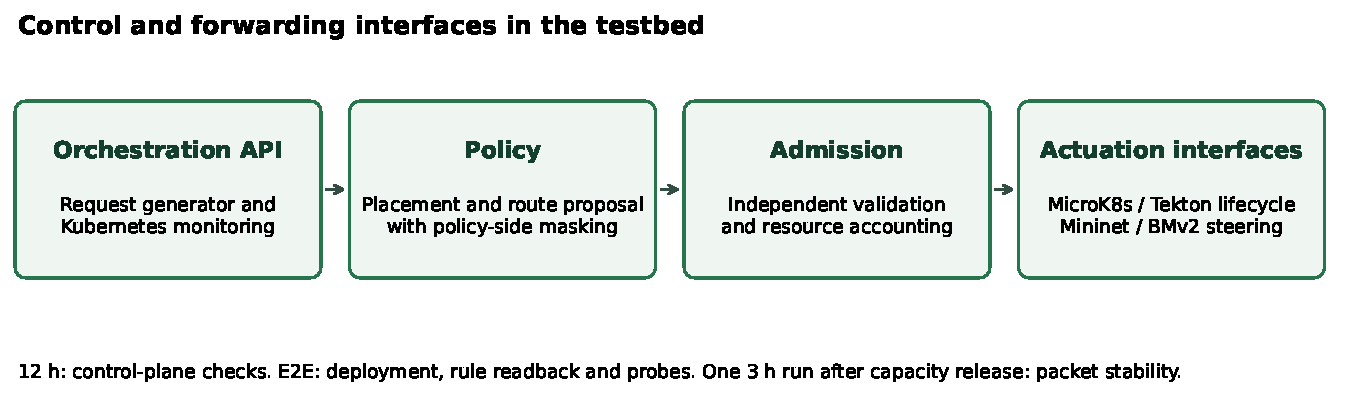
\includegraphics[width=\linewidth]{figs/testbed.pdf}
\caption{\rev{Hardware-in-the-loop testbed integrating AIO-Mesh runtime admission, cloud-native VNF lifecycle control, SRv6/P4 steering, and post-actuation monitoring.}}
\label{fig:testbed_architecture_eval}
\end{figure*}

\rev{HARP, Hybrid, and Heuristic use runtime admission; Greedy and DAI are diagnostic unprotected baselines. Table~\ref{tab:testbed_results} reports admission as a percentage of offered requests and MSD violations as a percentage of admitted requests. These rates are not request counts. Because policy and protection differ between rows, this HIL comparison alone does not isolate the effect of admission.}

\rev{Table~\ref{tab:testbed_results} reports zero observed admitted MSD violations for the protected configurations. Positive admitted MSD-violation rates in the unprotected configurations range from 6.4\% to 89.5\%. The simulation ablations in Table~\ref{tab:vietnam_ablation_summary} separately examine masking and admission.}

\begin{table}[!tb]
\centering
\caption{\rev{HIL admission / admitted MSD-violation rates (\%; mean across $N=10$ independent runs). Denominators within each run are offered / admitted requests, respectively; Greedy and DAI are unprotected.}}
\label{tab:testbed_results}
\renewcommand{\arraystretch}{1.08}
\setlength{\tabcolsep}{2pt}
\small
\resizebox{\linewidth}{!}{
\begin{tabular}{@{}lccccc@{}}
\toprule
\textbf{Algorithm} & \textbf{Normal} & \textbf{Elephant} & \makecell{\textbf{Topo}\\\textbf{stress}} & \makecell{\textbf{DDoS}\\\textbf{MBB}} & \textbf{Chaos} \\
\midrule
\textbf{HARP} & 100.0 / 0.0 & 72.4 / 0.0 & 22.6 / 0.0 & 24.2 / 0.0 & 10.8 / 0.0 \\
Hybrid runtime & 100.0 / 0.0 & 76.5 / 0.0 & 22.6 / 0.0 & 25.6 / 0.0 & 8.9 / 0.0 \\
Heuristic & 100.0 / 0.0 & 66.8 / 0.0 & 21.4 / 0.0 & 23.2 / 0.0 & 8.4 / 0.0 \\
Greedy & 100.0 / 0.0 & 58.4 / 18.6 & 22.6 / 77.4 & 26.5 / 67.5  & 8.4 / 78.4 \\
DAI & 93.6 / 6.4 & 51.8 / 21.4 & 9.8 / 89.5 & 19.2 / 76.2 & 6.2 / 80.5 \\
\bottomrule
\end{tabular}}
\end{table}

\rev{Under HIL Chaos, HARP reports 10.8\% acceptance with zero observed admitted MSD violations, compared with 8.9\% for Hybrid and 8.4\% for Heuristic. These observations apply to the tested pair-level checks and workload.}

\rev{A continuous 24-hour Hardware-in-the-Loop run evaluated long-term operational stability under dynamic background traffic, as summarized in Table~\ref{tab:hil_24h_stability}.}

\begin{table}[!tb]
\centering
\caption{\rev{24-hour HIL operational summary}.}
\label{tab:hil_24h_stability}
\renewcommand{\arraystretch}{1.10}
\small
\begin{tabularx}{\linewidth}{>{\raggedright\arraybackslash}Xr}
\toprule
\textbf{Operational metric} & \textbf{Reported value} \\
\midrule
Processed requests & 25,000 \\
Admitted and deployed & 18,150 (72.60\%) \\
CPU/memory rejections & 5,620 (22.48\%) \\
MSD rejections & 1,230 (4.92\%) \\
Observed admitted MSD violations & 0 \\
Controller/deployment failures & 0 \\
Telemetry/mask-refresh failures & 0 \\
Mean decision latency, first/last hour & 4.18 / 4.22 ms \\
\bottomrule
\end{tabularx}
\end{table}

\rev{The 24-hour continuous execution log was fully reconciled across all 25,000 processed requests (average arrival rate $\approx 0.29$ req/s). Exactly 18,150 requests ($N_{\text{adm}} = 18,150$, 72.60\%) were admitted and successfully deployed, 5,620 requests (22.48\%) were rejected due to CPU/memory limits, and 1,230 requests (4.92\%) were rejected due to SRv6 MSD limits ($N_{\text{viol}} = 0$, $R_{\text{viol}} = 0.0\%$). No controller or telemetry failures were recorded during the 24-hour run. Mean decision latency increased only slightly from 4.18~ms in the first hour to 4.22~ms in the last hour ($\Delta=0.04$~ms), indicating stable observed decision-processing performance over the evaluated period.}

\rev{To investigate the operational consequences of MSD overflow, a controlled injection uses a seven-SID realization against a configured depth limit of four. Table~\ref{tab:over_msd_injection} summarizes the protected and bypass outcomes.}

\begin{table}[!tb]
\centering
\caption{\rev{Over-MSD injection outcomes} (\(h_q=7\), \(m_v^{msd}=4\)).}
\label{tab:over_msd_injection}
\renewcommand{\arraystretch}{1.10}
\small
\begin{tabularx}{\linewidth}{p{1.6cm}XX}
\toprule
Metric & Unprotected & Protected \\
\midrule
Admission & Passed to actuation & Rejected \\
BMv2/P4 & Parser error reported & No rule installation \\
Counter/log & \texttt{msd\_violation\_drop} & \texttt{admission\_reject\_msd} \\
Packet loss & 100\% (Parser Drop) & 0\% (Fallback Route) \\
\bottomrule
\end{tabularx}
\end{table}

\rev{The injection demonstrates rejection of the tested over-depth configuration before actuation. Loss-free forwarding on the fallback route does not imply deployment of the rejected chain.}


\subsection{Scalability and Online Processing Overhead}
\label{subsec:scalability_path_sensitivity}

\rev{The scalability analysis considers substrate topologies ranging from 10 to 100 nodes. Table~\ref{tab:scalability_reported} reports mean decision-processing component timings, whose sum increases from 2.9 to 22.0~ms. These sums are not measured P95 decision-path latencies. Because topology size and active-chain count increase simultaneously, their individual contributions to processing overhead cannot be isolated. The reported validation timings cover pair-level admission checks but exclude full-chain realization, realization-time validation, and deployment operations.}


\begin{table}[!tb]
\centering
\caption{\rev{\rev{Decision-processing component timings} (ms); sum is not P95 latency.}}
\label{tab:scalability_reported}
\renewcommand{\arraystretch}{1.10}
\small
\resizebox{\linewidth}{!}{
\begin{tabular}{rrrrrrrr}
\toprule
$|V|$ & $|E|$ & Chains & State & Mask & Infer. & Valid. & Sum \\
\midrule
10 & 16 & 20 & 0.2 & 1.1 & 1.2 & 0.4 & 2.9 \\
25 & 45 & 50 & 0.4 & 2.8 & 1.8 & 0.6 & 5.6 \\
50 & 110 & 100 & 0.8 & 6.2 & 2.6 & 0.9 & 10.5 \\
100 & 240 & 200 & 1.5 & 14.8 & 4.2 & 1.5 & 22.0 \\
\bottomrule
\end{tabular}}
\end{table}

\begin{figure}[!tb]
\centering
% Reconstructed from Table scalability_reported; no inferred throughput or P95.
{\color{blue}
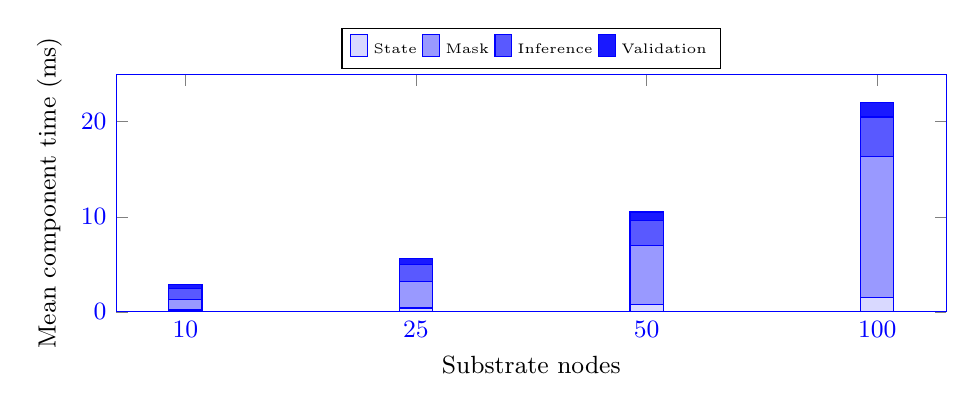
\begin{tikzpicture}
\begin{axis}[width=\linewidth,height=4.6cm,ybar stacked,bar width=12pt,symbolic x coords={10,25,50,100},xtick=data,ymin=0,ymax=25,xlabel={Substrate nodes},ylabel={Mean component time (ms)},label style={font=\small},legend style={font=\tiny,at={(0.5,1.02)},anchor=south,legend columns=4},axis line style={blue},tick label style={font=\small,text=blue}]
\addplot+[fill=blue!15,draw=blue] coordinates {(10,0.2) (25,0.4) (50,0.8) (100,1.5)};
\addplot+[fill=blue!40,draw=blue] coordinates {(10,1.1) (25,2.8) (50,6.2) (100,14.8)};
\addplot+[fill=blue!65,draw=blue] coordinates {(10,1.2) (25,1.8) (50,2.6) (100,4.2)};
\addplot+[fill=blue!90,draw=blue] coordinates {(10,0.4) (25,0.6) (50,0.9) (100,1.5)};
\legend{State,Mask,Inference,Validation}
\end{axis}
\end{tikzpicture}}
\caption{\rev{Mean decision-component timings from Table~\ref{tab:scalability_reported}. Stacked heights are component sums, not P95; actuation is excluded.}}
\label{fig:scalability_latency}
\end{figure}

\rev{The observed growth in mask processing time is compatible with the \(N^2\) action representation analyzed in Section~\ref{subsec:harp_complexity}. Nevertheless, end-to-end operational latency must include queueing, lifecycle deployment, readiness checks, SRv6/P4 actuation, and steering confirmation. These components cannot be inferred from inference time alone.}

\begin{table*}[!tb]
\centering
\caption{\rev{Concurrency-sweep results on the 10-node Vietnam topology. Arrival rate represents offered load. Decision-path P95 is distinct from component-delay sums and deployment latency}}
\label{tab:concurrency_sweep}
\small
\renewcommand{\arraystretch}{1.1}
\setlength{\tabcolsep}{4pt}
\begin{tabularx}{\textwidth}{*{6}{>{\centering\arraybackslash}X}}
\toprule
\shortstack[c]{Arrival rate\\(req/s)} &
\shortstack[c]{Active chains\\$\lvert\mathcal{M}_{\mathrm{active}}\rvert$} &
\shortstack[c]{Queue delay\\(ms)} &
\shortstack[c]{Reported P95\\decision (ms)} &
\shortstack[c]{Safe acceptance\\(\%)} &
\shortstack[c]{Admitted MSD\\violations (\%)} \\
\midrule
10 & 20 & 0.1 & 2.9 & $18.2^{\pm0.4}$ & $0.00^{\pm0.00}$ \\
50 & 50 & 0.3 & 3.4 & $18.1^{\pm0.5}$ & $0.00^{\pm0.00}$ \\
100 & 100 & 0.8 & 4.8 & $17.9^{\pm0.6}$ & $0.00^{\pm0.00}$ \\
250 & 200 & 2.5 & 8.5 & $17.5^{\pm0.7}$ & $0.00^{\pm0.00}$ \\
500 & 400 & 8.4 & 15.2 & $16.8^{\pm0.8}$ & $0.00^{\pm0.00}$ \\
1000\textsuperscript{*} & 800 & 29.5 & 38.6 & $14.2^{\pm1.1}$ & $0.00^{\pm0.00}$ \\
\bottomrule
\end{tabularx}
\vspace{2pt}
\parbox{\textwidth}{\footnotesize \textsuperscript{*}At an arrival rate of 1000 req/s, queue capacity saturation (\rev{\(Q_{\max}=1000\)}) triggers intentional tail-drops for low-priority non-SLA requests. \rev{No admitted MSD violations were observed at this offered load.}}
\end{table*}


\rev{Table~\ref{tab:concurrency_sweep} summarizes offered load, queue delay, and decision-path P95. These measurements distinguish request arrival from completed throughput and exclude lifecycle deployment.}

\rev{The finite candidate search rejects requests when no proposal satisfies the implemented checks. This behavior does not establish full-chain feasibility or exhaustiveness beyond the searched set.}

\subsection{Operational Interpretation, Overhead, and Limitations}
\label{subsec:operational_interpretation}

\rev{The results separate policy effectiveness from runtime enforcement: HARP's admission advantage depends on topology and workload, whereas the tested protected configurations show zero admitted MSD violations. The 2.9--22.0 ms component sums characterize decision processing, excluding deployment.}

\rev{The cost of the learned decision component follows the graph-encoding, \(N^2\)-logit actor, and local-mask complexity analyzed in Section~\ref{subsec:harp_complexity}. Deployment overhead includes Kubernetes/Tekton operations, readiness checking, SRv6/P4 rule installation, and steering confirmation, which are not captured by the policy-inference measurements. \rev{The component timings characterize HARP's decision path and do not establish a computational advantage over SAF-H.}}

\rev{The prototype has several limitations.} BMv2 validates parser-depth logic and control-plane behavior, but not ASIC line-rate forwarding. The workloads are synthetic and stress-oriented; production traces would strengthen external validity. Finally, the forecasting adapter is used as an operational trigger rather than as a separately evaluated prediction model. \rev{In addition, the implemented admission predicates operate on controller-visible state and a compact placement--routing action. They do not certify arbitrary full-chain SID-list realizations or guarantee atomic deployment across independent controllers. Make-before-break ordering likewise does not establish packet-level zero-downtime migration. Consequently, the evaluation supports conditional runtime enforcement under the tested implementation and workloads, rather than unconditional physical deployment safety.}

\section{Conclusion}
\label{sec:conclusion}
This paper presented AIO-Mesh, a hardware-safe AIOps orchestration framework for cloud-native service function chains over programmable SRv6/P4 data planes. The key design principle is to separate hard deployability constraints from soft operational objectives. HARP ranks placement--routing proposals, while policy-independent runtime admission checks modeled CPU, memory, and MSD constraints before actuation. \rev{By integrating graph-attention inference, feasibility-aware admission, Kubernetes/Tekton lifecycle management, and programmable steering, AIO-Mesh separates adaptive decisions from safety enforcement. Policy-side masking improves candidate selection, while runtime admission blocks proposals violating checked constraints before actuation.}

\rev{Evaluation across the Vietnam backbone, NSFNET, and GEANT2 demonstrates this separation. HARP improves safe acceptance over Greedy and DAI, while paired comparisons with SAF-H favor HARP in seven of nine configurations at Holm-adjusted \(p<0.05\). Under Burst Surge, HARP achieves $19.15\pm0.46\%$ and $50.25\pm0.44\%$ safe acceptance on Vietnam and GEANT2, respectively. The ablation results distinguish policy masking from runtime admission, while hardware-in-the-loop experiments report zero observed admitted MSD violations under protected execution. A continuous 24-hour testbed run processes 25,000 requests without observed admitted MSD violations, and the scalability analysis characterizes decision-processing overhead on topologies up to 100 nodes.}

The current prototype has several limitations. The programmable data plane is validated with BMv2 rather than production ASIC or smartNIC/DPU targets, and the workloads are synthetic stress scenarios rather than production traces. \rev{The evaluated safety scope is conditional on controller-visible state and the modeled predicates checked during pair-level admission and realization-time validation. These checks do not establish unconditional full-chain deployability, atomic cross-controller execution, or packet-level zero-downtime migration.} Future work will address full-chain realization, cross-controller consistency, and packet-level migration continuity \rev{on production-grade programmable infrastructures}.

\section*{Declaration of Competing Interest}
The authors declare that they have no known competing financial interests or personal relationships that could have appeared to influence the work reported in this paper.

\section*{Funding} 
\noindent This work was supported by the Ministry of Science and Technology of Vietnam through the National Science and Technology Program, under Project No.~KC.01.06/21-30.

\section*{Data and Code Availability}
The simulation scenarios, topology descriptions, workload configurations, testbed scripts, Mininet/BMv2 setups, SRv6/P4 steering scripts, Tekton pipeline definitions, and evaluation logs used in this study are publicly available at:
\url{https://github.com/uet-dis/AIO-Mesh/}.

\section*{Declaration of Generative AI and AI-Assisted Technologies in the Writing Process}
During the preparation of this work, the authors used generative AI and AI-assisted technologies to refine the scientific prose, improve readability, and polish LaTeX formatting. After using these technologies, the authors thoroughly reviewed and edited the content as needed and take full responsibility for the content of the published article.

\section*{CRediT Authorship Contribution Statement}
\textbf{Hanh P. Du}: Conceptualization, Methodology, Formal analysis, Validation, Writing -- original draft.
\textbf{Hung D. Hoang}: Software, Investigation, Testbed implementation, Visualization, Validation, Writing -- original draft.
\textbf{Thu H. Le}: Software, Data curation, Experimental evaluation, Visualization, Writing -- review \& editing.
\textbf{Tuan X. Le}: Software, Validation, Writing -- review \& editing.
\textbf{Giang L. Nguyen}: Formal analysis, Validation, Writing -- review \& editing.
\textbf{Hoa N. Nguyen}: Conceptualization, Methodology, Supervision, Project administration, Funding acquisition, Writing -- review \& editing.

\bibliographystyle{elsarticle-num}
\bibliography{refs}

\end{document}